%% 
%% Copyright 2007-2020 Elsevier Ltd
%% 
%% This file is part of the 'Elsarticle Bundle'.
%% ---------------------------------------------
%% 
%% It may be distributed under the conditions of the LaTeX Project Public
%% License, either version 1.2 of this license or (at your option) any
%% later version.  The latest version of this license is in
%%    http://www.latex-project.org/lppl.txt
%% and version 1.2 or later is part of all distributions of LaTeX
%% version 1999/12/01 or later.
%% 
%% The list of all files belonging to the 'Elsarticle Bundle' is
%% given in the file `manifest.txt'.
%% 
%% Template article for Elsevier's document class `elsarticle'
%% with harvard style bibliographic references

%% For review
\documentclass{interact}

\usepackage{epstopdf}% To incorporate .eps illustrations using PDFLaTeX, etc.
\usepackage{subfigure}% Support for small, `sub' figures and tables

\usepackage{natbib}% Citation support using natbib.sty
\bibpunct[, ]{(}{)}{,}{a}{}{,}% Citation support using natbib.sty
\renewcommand\bibfont{\fontsize{10}{12}\selectfont}% Bibliography support using natbib.sty

\theoremstyle{plain}% Theorem-like structures
\newtheorem{theorem}{Theorem}[section]
\newtheorem{lemma}[theorem]{Lemma}
\newtheorem{corollary}[theorem]{Corollary}
\newtheorem{proposition}[theorem]{Proposition}

\theoremstyle{definition}
\newtheorem{definition}[theorem]{Definition}
\newtheorem{example}[theorem]{Example}

\theoremstyle{remark}
\newtheorem{remark}{Remark}
\newtheorem{notation}{Notation}

%% For preview
% \documentclass[12pt,authoryear,times]{elsarticle}
% \usepackage[margin=1in]{geometry}

%% For including figures, graphicx.sty has been loaded in
%% elsarticle.cls. If you prefer to use the old commands
%% please give \usepackage{epsfig}

%% The amssymb package provides various useful mathematical symbols
\usepackage{amssymb}
%% The amsthm package provides extended theorem environments
\usepackage{amsthm}

%% The lineno packages adds line numbers. Start line numbering with
%% \begin{linenumbers}, end it with \end{linenumbers}. Or switch it on
%% for the whole article with \linenumbers.
\usepackage{lineno}
% \usepackage{esdiff}
\usepackage{xcolor}
\usepackage[colorlinks=true,citecolor=teal]{hyperref}
\usepackage{enumitem}
\usepackage{booktabs}
\usepackage{multirow}
\usepackage{makecell}
\usepackage{tabularx}

\renewcommand{\sectionautorefname}{Section}
\renewcommand{\subsectionautorefname}{Subsection}

%%% =====================
%%% Glossaries
%%% =====================
\usepackage[acronyms,shortcuts]{glossaries}
\newcommand{\acrcite}[1]{\glsentrylong{#1} \ifglshasfield{useri}{#1}{\citep[\glsentryshort{#1};][]{\glscurrentfieldvalue}}{}\glsunset{#1}}
\glsdisablehyper
\newacronym{dgp}{DGP}{data generation process}
\newacronym{rmse}{RMSE}{root mean square error}
\newacronym{mae}{MAE}{mean absolute error}
\newacronym{cv}{CV}{cross-validation}
\newacronym{aic}{AIC}{Akaike Information Criterion}
\newacronym{aicc}{AICc}{corrected Akaike Information Criterion}
\newacronym[user1={BrunsdonFotheringham-1996}]{gwr}{GWR}{Geographically Weighted Regression}
\newacronym[user1={FotheringhamYang-2017,LuBrunsdon-2017}]{mgwr}{MGWR}{Multiscale Geographically Weighted Regression}
\newacronym[user1={Goldstein-2011}]{hlm}{HLM}{Hierarchical Linear Model}
\newacronym[user1={HuHarris-2024}]{hgwr}{HGWR}{Hierarchical and Geographically Weighted Regression}
\newacronym{glsw}{GLSW}{group-level spatially weighted}
\newacronym{slr}{SLR}{simple-level random}
\newacronym{icc}{ICC}{intraclass correlation coefficient}
\newacronym[user1={Anselin-1995}]{lisa}{LISA}{local indicators of spatial association}
\newacronym{anova}{ANOVA}{analysis of variance}

\usepackage{mathshortcuts}
\usepackage{xspace}
\newcommand{\varn}[1]{\ifmmode\text{\textit{#1}}\else\textit{#1}\fi\xspace}
\newcommand{\Intercept}{\varn{Intercept}}
\newcommand{\Province}{\varn{Province}}
\newcommand{\QOESpend}{\varn{QOE.Spend}}
\newcommand{\QOESpendRatio}{\varn{QOE.Spend.Ratio}}
\newcommand{\QOESpendingPH}{\varn{QOE.Spend.PerHour}}
\newcommand{\QOESpendingph}{\varn{QOE.Spend.PerHour}}
\newcommand{\QOESpending}{\varn{QOE.Spend}}
\newcommand{\GDPPrimary}{\varn{GDP.Primary}}
\newcommand{\CPI}{\varn{CPI}}
\newcommand{\NumEnterprise}{\varn{Num.Enterprise}}
\newcommand{\TotalIncome}{\varn{Total.Income}}
\newcommand{\TotalSpending}{\varn{Total.Spending}}
\newcommand{\Engel}{\varn{Engel}}
\newcommand{\Pop}{\varn{Population}}
\newcommand{\PopHighEduMale}{\varn{Pop.High.Edu.Male}}
\newcommand{\PopHighEduFemale}{\varn{Pop.High.Edu.Female}}
\newcommand{\HighEducated}{\varn{Pop.High.Educated}}
\newcommand{\Gini}{\varn{Gini}}
\newcommand{\UrbanSpendTotal}{\varn{Urban.Spend.Total}}
\newcommand{\UrbanSpendFood}{\varn{Urban.Spend.Food}}
\newcommand{\Asset}{\varn{Asset}}
\newcommand{\Debt}{\varn{Debt}}
\newcommand{\HighEdu}{\varn{High.Edu.Parent}}
\newcommand{\Age}{\varn{Age}}
\newcommand{\QOETime}{\varn{QOE.Time}}
\newcommand{\prov}{\varn{prov}}
\newcommand{\geom}{\varn{geom}}
\newcommand{\GenderMale}{\varn{Gender.Male}}
\newcommand{\RegionUrban}{\varn{Region.Urban}}
\newcommand{\CultCentCountTotal}{\varn{Youth.Palace.Count}}
\newcommand{\UniversityRecruitRatio}{\varn{University.Recruit.Ratio}}
\newcommand{\GeneralEduBudget}{\varn{General.Edu.Budget}}
\newcommand{\NationalFiscalExpenditure}{\varn{National.Fiscal.Expenditure}}
\allowdisplaybreaks

\linespread{2}

\begin{document}


\articletype{RESEARCH ARTICLE}


\title{Testing Spatial Heterogeneity in Hierarchical and Geographically Weighted Regression: Theory, Simulation, and a Study of Extracurricular Education in China}

\author{
  \name{Yigong Hu\textsuperscript{a}\thanks{Corresponding author. Email: yigong.hu@hhu.edu.cn}, Richard Harris\textsuperscript{b}, and Richard Timmerman\textsuperscript{b}}
  \affil{
    \textsuperscript{a}College of Geography and Remote Sensing, Hohai University, Nanjing, Jiangsu, China. 211000.
    \textsuperscript{b}School of Geographical Sciences, University of Bristol, UK. BS8 1SS.
  }
}

\maketitle

\begin{abstract}
%% Text of abstract
\Gls{hgwr} models spatial hierarchical data by combining \gls{glsw}, fixed, and sample-level random effects. Although \gls{glsw} estimates are allowed to vary geographically, variation in an estimated coefficient surface does not by itself establish spatial heterogeneity because sampling error and spatial autocorrelation may produce similar patterns. We address this inferential gap by defining spatial heterogeneity through location-conditional distributions and by developing an effect-wise parametric bootstrap and an approximate $F$ test for the spatial heterogeneity of \gls{glsw} effects. Monte Carlo experiments with 200 fixed random locations assess calibration, power, effect specificity, and computational stability. At \gls{icc} 0.4, the effect-wise bootstrap has null rejection rates of 3.2\% and detects a heterogeneous effect in 96.9--100\% of usable repetitions while rejecting the accompanying constant effect in only 3.1--4.1\%. The corrected $F$ approximation is computationally inexpensive but remains liberal in several null settings and increasingly rejects the constant effect when another effect is heterogeneous. We then apply the framework to household investment in children's extracurricular courses in China, integrating household survey, provincial panel, geographic, and point-of-interest data. The application illustrates how heterogeneity testing can inform the allocation of provincial variables to \gls{glsw} or fixed effects, while the simulation results also show why evidence based only on the $F$ approximation should be interpreted cautiously.
\end{abstract}

%%Graphical abstract
% \begin{graphicalabstract}
%\includegraphics{grabs}
% \end{graphicalabstract}

%%Research highlights
% \begin{highlights}
% \item Research highlight 1
% \item Research highlight 2
% \end{highlights}

\begin{keywords}
%% keywords here, in the form: keyword \sep keyword

%% PACS codes here, in the form: \PACS code \sep code

%% MSC codes here, in the form: \MSC code \sep code
%% or \MSC[2008] code \sep code (2000 is the default)
Statistical inference; hypothesis test; spatial heterogeneity; bootstrap; hierarchical and geographically weighted regression; extracurricular education
\end{keywords}

\glsresetall
\linenumbers

%% main text
\section{Introduction}
\label{sec:introduction}

Data possesses immense value, and data analysis unveils numerous patterns in the world and society \citep{Bormida-2021,Al-SaiHusin-2022}, including spatial effects \citet{AnselinGriffith-1988,AnselinCho-2002,LegendreDale-2004,ParadinasIllian-2023,HeHe-2025}.
When examining spatially distributed data, discernible patterns in the data or their conditional values often indicate that observations from one location differ systematically (for instance, in their mean values) from those at other locations.
This connection between geographic context and measured outcomes is broadly described as spatial dependency: values are not distributed randomly or uniformly across the geographic domain \citep{Anselin-2010,Haining-2003}.
Tobler's First Law of Geography \citep{Tobler-1970} is frequently interpreted as articulating positive spatial autocorrelation, positing that proximate entities (or values) tend to exhibit greater similarity than those that are more distant.
Under this premise, a closer inspection of any subregion of the map should reveal localised clusters of relatively homogeneous values.
Alternatively, with a shift in emphasis, the same principle can be construed as an expression of spatial heterogeneity: if distant entities differ, then one should generally expect to observe systematic variations across the map, with different areas characterized by distinct attributes.
This implies that spatial autocorrelation and spatial heterogeneity, while interrelated, are conceptually distinct. 
One key distinction lies in their scale of manifestation. 
Spatial autocorrelation typically refers to localised patterns emerging, for example, from interactions among individuals or between species and their immediate surroundings \citep[p. 255]{FischerGetis-2010}.
In contrast, spatial heterogeneity may arise from broader contextual differences across regions, wherein varying local conditions foster divergent developmental pathways and evolutionary trajectories \citep{DutilleulLegendre-1993,ShiyomiTakahashi-2000,EscobedoNowak-2009,Long-2010}
A consequence of such divergent processes is that outcomes may vary substantially across a study area.
An aim of this paper is to define more precisely what is meant by spatial heterogeneity and how it differs from spatial autocorrelation. 
The motivation is to develop a test of spatial heterogeneity for a relatively new method of spatial analysis, which is \gls{hgwr}. 
However, the discussion of what is meant by spatial heterogeneity is more foundational, and will be of interest beyond the specific case study of \gls{hgwr}.

Spatial dependence has been widely understood and studied with the development of spatial statistics and tests of spatial autocorrelation,
whereas spatial heterogeneity has more recently been gaining increased attention \citep{ZhaiFeng-2023,HuLu-2022,HelbichBrunauer-2014,WangZhao-2018,ZhaoLiu-2021}, due to its prevalence in spatial data sets\footnote{
  The term ``spatial data sets'' here means data spanning a geographical study region, for which the location of the measurement as well as the measurement itself is recorded.
} \citep{LiuWang-2023-en,LokeChisholm-2022,ZhaoLiu-2021,YangFang-2019,WolfOshan-2018,Yuan-2016} and the resulting risk of ``ecological fallacy'' in the inference on individuals using globally constant relationship \citep{LokarZagar-2019,Openshaw-1984,TranmerSteel-1998,FieldhouseTye-1996}.
In addition to the spatial effects, spatial hierarchical structure also demonstrates significant influence on spatial data analysis,
such as failure on model fitting \citep{HuLu-2022} and spatial spillover effects \citep{DongHarris-2015a}.
We use ``spatial hierarchical data'' to refer to data that are products of a geographical process exhibiting spatial effects in its measurements, and that are structured in a way creating a grouping effect or hierarchy.
They are a consequence of what is measured, as well as how it is measured. 
As an example, in housing price analysis in China, properties are grouped by communities, and attributes from both properties and communities impact the prices \citep{HuHarris-2024,HuLu-2022}.
Such data are prevalent in various fields, including health, economy, and social sciences
\citep{ChenTruong-2012,BrunauerLang-2013,FeuilletCossart-2024,AielloRicotta-2016}.

To model spatial hierarchical data, special methods are necessary to account for its characteristics.
The \acrcite{hgwr} model is a synthesis of \acrcite{gwr} and \acrcite{hlm}.
To handle spatial hierarchical data,
\gls{hgwr} includes three types of effects: \gls{glsw} effects, fixed effects, and \gls{slr} effects.
\gls{glsw} and \gls{slr} effects allow for the possibility of spatial heterogeneity at the group and sample levels, respectively, while fixed effects capture globally constant influences (i.e. effects that do not vary geographically across the study region).
% A key restriction is that \gls{glsw} effects are applicable only to group-level variables, whereas \gls{slr} effects are restricted to sample-level variables.
% To estimate these effects, \gls{hgwr} employs a back-fitting algorithm and a maximum likelihood estimator \citep[BFML;][]{ChenLeung-2022}, enabling simultaneous estimation of all effects within the hierarchical structure.

However, at the time of writing, relatively little work has been undertaken to situate the model within a formal framework of statistical inference, particularly with respect to testing the significance of any spatial heterogeneity observed in estimates of \gls{glsw} effects.
As a hybrid of parametric and non-parametric methods \citep{HuHarris-2024,HuHarris-2024a}, \gls{hgwr} lacks a well-established inferential foundation.
The reasons for this are twofold.
When adopting a probability-based approach to inference, the hierarchical structure introduces additional complexity in deriving probability distributions compared to the hypothesis tests of \gls{gwr} \citep{LeungMei-2000}.
Conversely, if one turns to resampling-based bootstrap methods \citep{MooneyDuval-1993,DelgadoManteiga-2001} a more fundamental question emerges: what precisely is the object of inference in the context of spatial heterogeneity?

Unlike spatial dependence that Moran's I \citep{Moran-1950,LiCalder-2007} and other well-known methods can quantify, spatial heterogeneity is challenging to be quantified, although there have been some attempts to do so \citep{TranPearson-2022}.
As spatial heterogeneity and spatial dependence often happen together, Moran's I and, in particular, \acrcite{lisa} ---
measures of spatial dependence that are estimated for parts of the study regions and not just for the study region as a whole ---
are sometimes employed to identify potential spatial heterogeneity \citep{JacksonHuang-2009,ZhangLin-2016}.
When \gls{gwr} is used to model spatially-varying regression relationships, one may then analyse the spatial heterogeneity in these relationships using either an $F$-test \citep{LeungMei-2000} or a bootstrap test \citep{HarrisBrunsdon-2017}.
For hierarchical or grouped data, \gls{anova} and \gls{hlm} are feasible methods \citep{DutilleulLegendre-1993,FotheringhamBrunsdon-2010,LignierJarvis-2024,KirkbrideStochl-2015} in addition to caterpillar plots visualising intraclass correlation in data grouped by geographical locations.
Geodetector \citep{WangZhang-2016,ZhaoLiu-2021,HuoSun-2021} offers a method to detect stratified heterogeneity in spatial data for finding homogeneous regions.
However, these methods need to meet certain assumptions to be applied.
Methods using Moran's I and \gls{lisa} assume that spatial heterogeneity arises from autocorrelation, while \gls{anova} or \gls{hlm} rely on grouping or repeated observations \citep{HuLu-2022,HuHarris-2024}.
Geodetector focus on uncovering categorical driving factors for numerical data, resulting in limitations of data types.

At heart is a more fundamental problem --- the absence of a widely accepted and formalised definition of spatial heterogeneity itself.
Whether concerning random variables or \gls{glsw} effects within the \gls{hgwr} model, equating spatial variation with spatial heterogeneity is not always appropriate.
At the very least, such variation may stem from random error.
Conversely, if spatial variation in the data is driven by spatial autocorrelation, it does not necessarily constitute spatial heterogeneity in the sense typically implied by local models.

To fill this gap, after introducing the \gls{hgwr} model, we clarify what constitutes spatial heterogeneity in this study, as well as the specific form of spatial heterogeneity that we aim to test.
\citet{LiuWang-2023-en} suggest viewing (geographical) space as an accumulation of fields.
In line with this theory, we conceptualise variables as randomly distributed within these fields, named ``spatial random variables''.
A spatial random variable is a conditional random variable where the location serves as the condition.
Yet, fields can be very complex and difficult to parameterize.
In this case, non-parametric methods, such as kernel density estimation, are applicable \citep{Tran-1990,HyndmanBashtannyk-1996,LuHu-2025}.
% Spatial heterogeneity exists when a variable's conditional distribution varies across locations.
This definition identifies spatial constancy as the relevant null hypothesis for the \gls{glsw} effects in \gls{hgwr}.
We evaluate that null hypothesis using bootstrap and distribution-based methods, thereby assessing whether the variation in an estimated \gls{glsw} effect is greater than would be expected under a spatially constant relationship.

The need for this distinction is especially clear in applied studies where variables are measured at more than one level.
We illustrate the problem using family investment in children's extracurricular courses, an important component of quality-oriented education (QOE) in China.
Participation and expenditure reflect household circumstances, while the availability and price of educational resources are shaped by provincial economic and policy contexts.
A mapped \gls{hgwr} coefficient can suggest that a provincial association differs geographically, but policy interpretation requires evidence that the variation is greater than would be expected under a spatially constant effect.
The case study therefore serves two purposes: it illustrates how a heterogeneity test can guide the choice between \gls{glsw} and fixed effects, and it shows how simulation evidence about calibration qualifies the interpretation of mapped educational inequalities.

This paper makes three contributions.
First, it formalises strong and weak spatial heterogeneity using location-conditional distributions and distinguishes spatial non-stationarity from spatial autocorrelation.
Second, it develops an effect-wise parametric bootstrap and a distribution-based approximate $F$ test for \gls{glsw} effects in \gls{hgwr} and uses Monte Carlo experiments to examine their calibration, power, effect specificity, and computational behaviour.
Third, it provides an empirical study in which approximate heterogeneity screening is integrated into effect specification rather than applied only after estimation, thereby connecting the methodological evaluation to household- and province-level correlates of extracurricular education investment.

The remainder of this paper will be organised as follows.
\autoref{sec:hgwr} outlines the mathematical foundations of the \gls{hgwr} model and identifies the \gls{glsw} effects as the object of inference.
\autoref{sec:spatial-heterogeneity} then presents our definitions of spatial heterogeneity and analyses how these definitions lead to a testable null hypothesis.
\autoref{sec:glsw-test} develops bootstrap and distribution-based $F$ tests for \gls{glsw} effects and assesses their effectiveness by simulation.
\autoref{sec:qoe-case} applies the framework to extracurricular education investment in China.
Finally, \autoref{sec:conclusion} concludes with the methodological findings, substantive implications, and limitations.

\section{Hierarchical and Geographically Weighted Regression}\label{sec:hgwr}

In addition to spatial analysis of individual variables, examining the relationships among multiple variables is often a more critical issue.
Due to the existence of spatial heterogeneity, local-form regression models \citep{FotheringhamBrunsdon-2010} analysing non-stationary relationships are popular with geographers, like \gls{gwr} \citep{HelbichBrunauer-2014,FanSong-2021,TranPearson-2022} and \gls{hlm} \citep{WuHou-2011,KirkbrideStochl-2015,WangJiang-2021}.
As a combination of \gls{gwr} and \gls{hlm}, the \gls{hgwr} model overcomes the limitations of the two models, such as the risk of singular matrix in \gls{gwr} and the inability to model spatial heterogeneity for group-level variables in \gls{hlm} \citep{HuHarris-2024}.
However, methods for testing the significance of spatial heterogeneity of the non-stationary relationships have been developed for \gls{gwr} via bootstrapping or $F$-test \citep{LeungMei-2000,MeiXu-2016,HarrisBrunsdon-2017} and \gls{hlm} \citep{GelmanHill-2006,Goldstein-2011},
while \gls{hgwr} lacks such methods.

Developing a hypothesis test for spatial heterogeneity in \gls{hgwr} is challenging due to the model's complexity.
At minimum, it is important to establish that the variation in \gls{glsw} effect estimates differs from the variation produced by the random component of the model.
To achieve this goal, starting from reviewing the basis of this model is essential.
This section summarises the definition and estimation of the \gls{hgwr} model, as the bootstrap method requires resampling according to the hierarchical error structure, and the $F$-test requires the \gls{glsw} estimator and its hat matrix.
After the model and its estimator are introduced, the next section defines the exact form of spatial heterogeneity to be tested.

\subsection{Definition}

% The \gls{hgwr} model \citep{HuHarris-2024} integrates geographically weighted regression and hierarchical modelling.
In a two-level \gls{hgwr} model, variables are classified as either group level or sample level, and their effects can be fixed or varying.
For sample $i$ in group $j$ from a data set of $n$ samples across $m$ groups, the \gls{hgwr} model can be expressed as \eqref{equ:hgwr-model-pointwise},
\begin{equation}\label{equ:hgwr-model-pointwise}
  y_{ij} = \vG_{ij}\vgamma_{j} + \vX_{ij}\vbeta + \vZ_{ij}\vmu_{j} + \epsilon_{ij}
\end{equation}
where $y_{ij}$ is the dependent variable of the sample;
$\vG_{ij}$ represents the group-level independent variables with spatially heterogeneous effects, $\vgamma_{j}$;
$\vX_{ij}$ includes group-level or sample-level independent variables of fixed effects, $\vbeta$;
$\vZ_{ij}$ denotes the sample-level independent variables of random effects, $\vmu_{j}$, and $\vmu_{j} \sim \vN(\vzero, \sigma^2\vD)$ with $\vD$ the variance-covariance matrix;
$\epsilon_{ij}$ represents the random error of the sample,
and $\epsilon_{ij} \sim N(0, \sigma^2)$, with $\sigma$ the variance.
$\vG_{ij}$, $\vX_{ij}$, $\vZ_{ij}$ are row vectors like
\begin{equation*}
  \vG_{ij} = \left(g_{ij1}, g_{ij2}, \cdots, g_{ijh}\right),
  \vX_{ij} = \left(x_{ij1}, x_{ij2}, \cdots, x_{ijp}\right),
  \vZ_{ij} = \left(z_{ij1}, z_{ij2}, \cdots, z_{ijq}\right)
\end{equation*}
with $h,p,q$ are the number of \gls{glsw}, fixed, and \gls{slr} effects, respectively.
These vectors are stacked for all samples and groups to form $\vG,\vX,\vZ$ as follows,
\begin{equation*}
  \vG = \begin{pmatrix}
    \vG_1 \\ \vG_2 \\ \vdots \\ \vG_m
  \end{pmatrix},
  \vG_j = \begin{pmatrix}
    \vG_{1j} \\ \vG_{2j} \\ \vdots \\ \vG_{n_{1}j} \\
  \end{pmatrix},
  \vX = \begin{pmatrix}
    \vX_1 \\ \vX_2 \\ \vdots \\ \vX_m
  \end{pmatrix},
  \vX_j = \begin{pmatrix}
    \vX_{1j} \\ \vX_{2j} \\ \vdots \\ \vX_{n_{1}j} \\
  \end{pmatrix},
\end{equation*}
\begin{equation*}
  \vZ = \begin{pmatrix}
    \vZ_1 & & & \\ 
    & \vZ_2 & & \\ 
    & & \ddots & \\ 
    & & & \vZ_m
  \end{pmatrix},
  \vZ_j = \begin{pmatrix}
    \vZ_{1j} \\ \vZ_{2j} \\ \vdots \\ \vZ_{n_{1}j} \\
  \end{pmatrix}.
\end{equation*}
Similarly, the vectors $\vgamma_j$ and $\vmu_j$ can also be vertically stacked, denoted by $\vgamma$ and $\vmu$, respectively.
The \gls{hgwr} model can be expressed in the matrix from, as shown in \eqref{equ:hgwr-model},
\begin{equation}\label{equ:hgwr-model}
  \vy = \diag(\vG\vgamma) + \vX\vbeta + \vZ\vmu + \vepsilon
\end{equation}
where $\vy$ is a column vector of all dependent variable values,
$\vepsilon$ is a column vector of all random errors,
and $\diag(\vG\vgamma)$ represents the diagonal elements of blocked matrix $\vG\vgamma$, i.e.,
\begin{equation*}
  \vG = \left(\begin{array}{c}
    \vG_1 \\\hline
    \vG_2 \\\hline
    \vdots \\\hline
    \vG_m
  \end{array}\right),
  \vgamma = \left(\begin{array}{c|c|c|c}
    \vgamma_1 & \vgamma_2 & \cdots & \vgamma_m
  \end{array}\right),
  \diag(\vG\vgamma) = \begin{pmatrix}
    \vG_1\vgamma_1 \\
    \vG_2\vgamma_2 \\
    \vdots \\
    \vG_m\vgamma_m \\
  \end{pmatrix}.
\end{equation*}

\subsection{Estimator}

A back-fitting and maximum likelihood (BFML) estimator is applied to estimate effects, $\vgamma,\vbeta,\vmu$.
Each $\vgamma_{j} (j=1,2,\cdots,m)$ in $\vgamma$ is estimated through a \gls{gwr}-like method by borrowing information from its geographical neighbours, using a kernel function $k$ with a parameter called bandwidth, $b$.
These are specified like the standard \gls{gwr} methods \citep{ComberBrunsdon-2022}.
The parameters $\vbeta$ and $\vmu$ are estimated using the maximum likelihood estimator.
After several iterations, all effects are properly estimated.
For the \gls{hgwr} model described above, the BFML estimator follows this procedure.

\begin{enumerate}[label=\textbf{Step \arabic*.}, left=0.5em, itemindent=2em]
\item Initialise. Set $\hat{\vD}^{(0)} = \vI$, $\hat{\vbeta}^{(0)} = 0$. Then let $\hat{\vV}^{(0)}=\vZ\hat{\vD}^{(0)}\vZ\T+\vI$.

\item Estimate \gls{glsw} effects.
Construct $\vy_g^{(t)}=\vy-\vX\hat{\vbeta}^{(t-1)}$.
Regard $\vZ\vmu$ as a part of random errors.
For $j$-th location $\vu_j$, by applying a \gls{gwr}-like method, $\hat{\vgamma}$ there can be estimated as \eqref{equ:bfml-glsw-estimator},
\begin{equation}\label{equ:bfml-glsw-estimator}
  \hat{\vgamma}_j^{(t)}
  = \left[\vG\T\vW_j\left(\vV^{(t)}\right)^{-1}\vG\right]^{-1} \left[\vG\T\vW_j\left(\vV^{(t)}\right)^{-1}\vy_g^{(t)}\right] 
  = (\vg\vw_j\vg')^{-1}(\vg\vw_j\vy'_{g})
\end{equation}
where $\vg=(\vg_1\T , \vg_2\T, \cdots, \vg_m\T)\T$,
$\vg_i=(g_{i1},g_{i2},\cdots,g_{ik})$,
$\vg'=\vV_{j\Sigma}^{-1}\vg $,
$\vy'_{g}=\vV_{j\Sigma}^{-1}\vy_g$,
and $\vV_{j\Sigma}^{-1}=1_{j}\T\vV_{j}^{-1}$.
The spatial weighting matrix $\vw(\vu)$ is calculated according to the coordinates of groups.

\item Estimate fixed effects.
With the estimated $\hat{\vgamma}^{(t)}$, let $\vy_h^{(t)}=\vy - \diag(\vG\hat{\vgamma})$, and $\vbeta$ can be estimated by the generalised weighted least squares estimator.

\item Estimate covariance of \gls{slr} effects, $\vD$, and variance of random errors, $\sigma^2$, denoted by $\hat{\vD}^{(t)}$ and $\hat{\sigma}^{(t)}$.

\item Estimate values of random effects.
After obtaining $\hat{\vD}^{(t)}$ and $\sigma^{2(t)}$ in iteration $t$, random effects can be computed as $\hat{\vmu}^{(t)} = \hat{\vD} \vZ\T\hat{\vV}^{-1}\left(\vy-\vX\hat{\vbeta}\right)$.

\item Compute the sum of squared residuals.
If it doesn't change significantly than that in previous iteration, terminate iteration; otherwise, set $t=t+1$ and return to step 2.
\end{enumerate}

In Step 2, it is common to calculate a so-called ``hat matrix'', $\vS$, such that $\hat{\vy}_g = \vS\vy_g$.
For the $i$-th sample in the $j$-th group, the corresponding row vector of $\vS$, denoted by $\vS_i$ is given by \eqref{equ:bfml-glsw-hatmat-row},
\begin{equation}\label{equ:bfml-glsw-hatmat-row}
  % \vS_i = \left[\vG\T\vW(\vu_i)\left(\vV^{(t)}\right)\I\vG\right]\I
  % \left[\vG\T\vW(\vu_i)\left(\vV^{(t)}\right)\I\right]
  \vS_{ij} = \left(\vg\vw_j\vg'\right)\I \vg\vw_j\vV_{i\Sigma}\I \;.
\end{equation}
The full form of $\vS$ is defined by stacking all $\vS_{ij} (i=1,2,\cdots,n;j=1,2,\cdots,m)$ vertically, as shown in \eqref{equ:bfml-glsw-hatmat},
% \begin{equation}\label{equ:bfml-glsw-hatmat}
%   \vS = \begin{pmatrix}
%     \vS_{11} \\
%     \vS_{12} \\
%     \vdots \\
%     \vS_{1n_1} \\
%     \vdots \\
%     \vS_{m1} \\
%     \vS_{m2} \\
%     \vdots \\
%     \vS_{mn_m} \\
%   \end{pmatrix} = \begin{pmatrix}
%     \left(\vg\vw(\vu_1)\vg'\right)\I \vg\vw(\vu_1)\vV_{1\Sigma}\I \\
%     \left(\vg\vw(\vu_1)\vg'\right)\I \vg\vw(\vu_1)\vV_{1\Sigma}\I \\
%     \vdots \\
%     \left(\vg\vw(\vu_1)\vg'\right)\I \vg\vw(\vu_1)\vV_{1\Sigma}\I \\
%     \vdots \\
%     \left(\vg\vw(\vu_m)\vg'\right)\I \vg\vw(\vu_m)\vV_{m\Sigma}\I \\
%     \left(\vg\vw(\vu_m)\vg'\right)\I \vg\vw(\vu_m)\vV_{m\Sigma}\I \\
%     \vdots \\
%     \left(\vg\vw(\vu_m)\vg'\right)\I \vg\vw(\vu_m)\vV_{m\Sigma}\I
%   \end{pmatrix} \;.
% \end{equation}
\begin{equation}\label{equ:bfml-glsw-hatmat}
  \vS = \begin{pmatrix}
    \vS_{1} \\ \vS_{2} \\ \vdots \\ \vS_{m}
  \end{pmatrix},
  \vS_{j} = \begin{pmatrix}
    \left(\vg\vw(\vu_j)\vg'\right)\I \vg\vw(\vu_j)\vV_{j\Sigma}\I \\
    \left(\vg\vw(\vu_j)\vg'\right)\I \vg\vw(\vu_j)\vV_{j\Sigma}\I \\
    \vdots \\
    \left(\vg\vw(\vu_j)\vg'\right)\I \vg\vw(\vu_j)\vV_{j\Sigma}\I
  \end{pmatrix} \;.
\end{equation}

The hat matrix will be important in deriving probability-based heterogeneity tests.
At this stage, however, the model only provides spatially varying estimates $\hat{\vgamma}_j$.
Whether their variation should be interpreted as spatial heterogeneity depends on the definition and null hypothesis developed in the next section.

\section{Spatial heterogeneity}
\label{sec:spatial-heterogeneity}

The preceding section shows that \gls{hgwr} allows the \gls{glsw} effect $\vgamma_j$ to vary among locations.
However, such variation is a property of the estimator and is not itself sufficient evidence of spatial heterogeneity.
The importance of spatial heterogeneity as a spatial effect has been widely recognised \citep{Anselin-2010,ShuPei-2019,ComberBrunsdon-2022}.
However, its description remains largely conceptual, suggesting that the characteristics of a geographical entity vary across different locations.
Researchers may sometimes find it challenging to differentiate spatial heterogeneity from spatial dependency, as the two often appear as two facets of the same phenomenon \citep{Anselin-2010}.
While methods such as \gls{lisa} and \gls{gwr} are available for analysing spatial heterogeneity,
they do not fully capture the essence of spatial heterogeneity or clearly distinguish it from spatial dependence.
Indeed, many of these methods presuppose the existence of spatial dependence as a starting premise.
Consequently, spatial heterogeneity remains elusive --- a presence observable but not easily quantified.
Before presenting a hypothesis testing method for spatial heterogeneity, we first need to establish a formal definition.

\subsection{Strong and weak spatial heterogeneity}

We assume that space is filled by many kinds of fields.
Each field $f$ maps the location $\vU$ to a geographical phenomenon or entity $X$ \citep{LiuWang-2023-en,LiuYao-2020-en}, represented by $f: \vU \rightarrow X$, where $\vU \in \mathbb{R}^m$, $m$ is the number of dimensions, and $X$ can be any value, vector or tuple relate to the geographical phenomenon or entity.
In this paper, we focus specifically on scalar-type $X$.
For clarity, we will refer to what X represents as an ``object''.
Note that $\vU$ is used to locate the object.
It can range from two dimensions (for geographical objects) to three dimensions (for spatial-temporal objects), or even four dimensions \citep[spatial interaction data][]{LiuYao-2020-en,KordiFotheringham-2016}.
Accordingly, we can express $X$ as the outcome of function $f$, i.e., $X = f(\vU)$.
However, in many real-world situations, the relationship between $X$ and $\vU$ may not be that deterministic, as $X$ can be a random variable.
In such cases, we define a spatial random variable $X$ as specified in \autoref{def:spatial-random-variable}.

\begin{definition}[Spatial random variable]
  \label{def:spatial-random-variable}
  Let random variable $\vU$ denote the location in the space $R \subseteq \mathbb{R}^m$ in the $m$-dimension space, and $X$ represent an event that happens in $R$.
  If the value of $X$ obeys the conditional distribution $f$ under the condition of $\vU$, i.e.,
  \begin{equation}
    X \sim f_{X|\vU}(x|\vu)
  \end{equation}
  where $x$ and $\vu$ are values of $X$ and $\vU$, respectively,
  then $X$ is a ``spatial random variable''.
\end{definition}

This definition permits spatial random variables to assume different values at various locations. 
Thus, variations in values do not necessarily indicate spatial heterogeneity, as they may be independently and identically distributed, which is still considered ``homogeneous.''
Only when changes in the probability density function across spatial locations lead to variations in the values of the random variable can they be deemed heterogeneous.
Thus, spatial heterogeneity is defined by \autoref{def:spatial-heterogeneity}.

\begin{definition}[Spatial heterogeneity] \label{def:spatial-heterogeneity}
  Let $\vU$ denote the random variable of the location of another random variable $X \sim f_{X|\vU}(x|\vu)$.
  For any two possible values of $\vU$, denoting $\vu_1,\vu_2$, there is spatial heterogeneity in $X$ when $f(x|\vu_1) \neq f(x|\vu_2)$; by contrast, there is no heterogeneity in $X$ when $f(x|\vu_1) = f(x|\vu_2)$ for every two possible values of $\vU$.
\end{definition}

There are two issues in \autoref{def:spatial-heterogeneity}.
According to this definition, it is nearly impossible for $X$ to exhibit no spatial heterogeneity,
making it a particularly stringent definition.
However, this strictness is acceptable since spatial heterogeneity is common.
The second issue pertains to scale: a geographical object exhibits heterogeneity only at certain scales.
For instance, climate may appear homogeneous within a city but heterogeneous on a global scale.
To address this, we define weak spatial heterogeneity by \autoref{def:spatial-heterogeneity-weak}.

\begin{definition}[Weak spatial heterogeneity]
  \label{def:spatial-heterogeneity-weak}
  Let random variable $\vU$ denote the location of another random variable $X \sim f_{X|\vU}(x|\vu)$ in $m$-dimension space $\mathbb{R}^m$.
  $R_1,R_2 \subseteq \mathbb{R}^m$ are any two consecutive fields where $R_1 \cup R_2 \neq R_1 \cap R_2$.
  For all $\vu_i,\vu_j \in R_1$, if $f(x|\vu_i)$ and $f(x|\vu_j)$ are statistically similar, there is no spatial heterogeneity in $X$ in $R_1$ (i.e., $X$ is spatial homogeneous in $R_1$).
  If $X$ is spatial homogeneous in $R_1$ and $R_2$, but $\vu_k \in R_2$ exists making $f(x|\vu_i)$ and $f(x|\vu_k)$ are statistically different, there is spatial heterogeneity in $X$ in $\mathbb{R}^m$.
\end{definition}

In \autoref{def:spatial-heterogeneity-weak}, we use the terms ``statistically similar'' and ``statistically different'' in place of ``equal'' and ``nonequal''.
To measure the statistical difference, we can apply hypothesis tests such as \gls{anova} \citep{Gelman-2005} or likelihood ratio test \citep{Woolf-1957}.
The ranges of $R_1$ and $R_2$ are controlled by the spatial scale of $X$.
This definition is more practical, as it permits variance within a group while still considering the set of all groups to exhibit spatial heterogeneity.
Therefore, we can choose a small area that presents no spatial heterogeneity as the fundamental unit for spatial analysis, in which samples are i.i.d. to a certain distribution.

However, a problem lies in that the conditional distribution $f(x|\vu)$ is typically unknown and often must be observed and estimated.
For example, air quality can be forecasted using models like the autoregressive integrated moving average model \citep{KumarJain-2010,AbhilashThakur-2018}.
Such forecasts generally provide the expectation, variance, or both of $X$, with the distribution represented by these indicators.
Under the condition of \autoref{def:spatial-random-variable}, the expectation of $X$ is the conditional expectation under $\vU$, i.e., $\conde{X}{\vU}$, and its variance is the conditional variance under $\vU$, i.e., $\condvar{X}{\vU}$, expressed as
\begin{equation*}
  \condvar{X}{\vU} = \conde{X^2}{\vU} - \left(\conde{X}{\vU}\right)^2
\end{equation*}
Compared to estimating the complete distribution of the random variable $X$, estimating its mean and variance is often more feasible.
Therefore, in practice, we primarily determine whether a variable exhibits spatial heterogeneity by observing its conditional mean and variance.
According to conditional density regression theories \citep{HyndmanBashtannyk-1996}, we know that
$\left.X \middle|(\vU=\vu)\right. = r(\vu) + \epsilon$ where $r(\vu)$ is the conditional mean.
According to the Nadaraya-Watson estimator \citep{Nadaraya-1964,Watson-1964}, $r(\vu)$ can be estimated by
\begin{equation}\label{equ:densityreg-neldermead}
  \hat{r}(\vu) = \sum_{j=1}^n w_j(\vu) X_j
\end{equation}
where
\begin{equation*}
  w_j(\vu) = \frac{
    K\left( \frac{\left\Vert \vu - \vu_j \right\Vert}{b_{\vu}} \right)
  }{
    \sum_{l=1}^n K\left( \frac{\left\Vert \vu - \vu_l \right\Vert}{b_{\vu}} \right)
  } \; ,
\end{equation*}
$K$ is a real, integrable, non-negative, and even kernel function,
and $b_{\vu}$ is the bandwidth.
Correspondingly, the estimated variance $X$ at $\vU = \vu$, $\hat{v}(\vu)$ is denoted by \citep{HallCarroll-1989},
\begin{equation}
  \hat{v}(\vu) = \sum_{j=1}^n w_j(\vu) \left[ X_j - \hat{r}(\vu) \right]^2 .
\end{equation}

The Nadaraya-Watson estimator can be seriously biased at samples near the boundary of the field, but local polynomial estimator overcomes this gap \citep{WangMei-2008,ZhaoZhang-2018}.
By assuming $r(\vu)$ is $p$-th order differentiable nearby $\vu_0$, we can express $r(\vu)$ as the Taylor expansion at $\vu$ according to \eqref{equ:densityreg-polynomial-taylor}
% \begin{equation}
\begin{multline}\label{equ:densityreg-polynomial-taylor}
  r(\vu) \approx r(\vu_0) + \sum_{v=1}^m \frac{r_v^{(1)}(\vu_0)}{1\!} (u_v - u_{0v}) + \sum_{v=1}^m \frac{r_{v}^{(2)}(\vu_0)}{2\!} (u_v - u_{0v}) + \cdots \\
  + \sum_{v_1=1}^m \frac{r_{v_1 v_2 \cdots v_p}^{(p)}(\vu_0)}{p\!} (u_{v} - u_{0 v}) + \cdots
\end{multline}
% \end{equation}
where $r_v^{(i)}$ is the $i$-th order partial derivative of $r$ with respect to the $v$-th dimension of $\vu$,
and $u_v,u_{0v}$ are the $v$-th dimensions of $\vu$ and $\vu_0$, respectively.
If we truncate \autoref{equ:densityreg-polynomial-taylor} at the $p$-th order,
the Taylor expansion becomes a $p$-th order polynomial of $\vu$, as
\begin{equation}\label{equ:densityreg-polynomial-poly}
  r(\vu) \approx r(\vu_0) + \sum_{d=1}^{p} \sum_{v=1}^{m} \xi_{d,v}(\vu)(u_v - u_{0v})^d
\end{equation}
where $\xi_{d,v}(\vu) = \frac{r_v^{(d)}(\vu_0)}{d\!}$.
Then we can estimate the coefficients of the Taylor expansion by minimizing the weighted least squares error as
\begin{equation}\label{equ:densityreg-polynomial}
  \hat{r}(\vu) = \sum_{i=1}^n \left[ X_i - \sum_{d=1}^{p}\sum_{v=1}^{m} \xi_{d,v}(\vu) (u_{iv} - u_{0v})^d \right]^2 K_h(vu_i - \vu) \;.
\end{equation}
Constructing vector $\vX = \left( X_1, X_2, \cdots, X_n \right)$ and matrix
\begin{equation*}
  \vD = \begin{pmatrix}
    1 & d_{11} & d_{12} & \cdots & d_{1m} & \cdots & d_{11}^p & d_{12}^p & \cdots & d_{1m}^p \\
    1 & d_{21} & d_{22} & \cdots & d_{2m} & \cdots & d_{21}^p & d_{22}^p & \cdots & d_{2m}^p \\
    \vdots & \vdots & \vdots & \ddots & \vdots & \vdots & \vdots & \ddots & \vdots \\
    1 & d_{n1} & d_{n2} & \cdots & d_{nm} & \cdots & d_{n1}^p & d_{n2}^p & \cdots & d_{nm}^p
  \end{pmatrix} \; ,
\end{equation*}
with $d_{iv} = u_{iv} - u_{0v}$,
the estimates of all $\xi$ can be expressed as
\begin{equation}
  \hat{\vxi}(\vu) = \left( \vD\T \vW(\vu) \vD \right)\I \vD\T \vW(\vu) \vX
\end{equation}
where $\vxi(\vu) = \left(r(\vu_0), \xi_{1,1}(\vu), \cdots, \xi_{1,m}(\vu), \xi_{p,1}(\vu), \cdots, \xi_{p,m}(\vu)\right)$, and
\begin{equation*}
  \vW(\vu) = \begin{pmatrix}
    K_h(\vu_1 - \vu) & & & \\
    & K_h(\vu_2 - \vu) & & \\
    & & \ddots & \\
    & & &  K_h(\vu_n - \vu)
  \end{pmatrix}
\end{equation*}
Thus, the estimates of $r(\vu_0)$ is the first element of $\hat{\vxi}(\vu)$.
In most cases, the results of local polynomial estimation are more accurate than those of the Nadaraya-Watson estimator \citep{ZhaoZhang-2018}.



\subsection{Spatial non-stationarity and spatial autocorrelation}

Although \autoref{def:spatial-heterogeneity-weak} offers relatively lenient conditions, practical application remains limited due to the unknown nature of the distribution function.
Below, we focus on a special case where $X$ is a normally distributed random variable.
In this scenario, spatial heterogeneity may be reflected in the mean and variance of $X$.
Under the assumption of Tobler's ``first law of geography'' being true \citep{Tobler-1970}, such spatial heterogeneity ultimately manifests as ``spatial non-stationarity'' and ``spatial autocorrelation''.

\begin{definition}[Spatial non-stationarity] \label{def:spatial-nonstationarity}
  If the value of a random variable $X$ on a field of location $\vu$, denoted by $g$, can be expressed as
  \begin{equation}
    X = g(\vu) + \epsilon
  \end{equation}
  where $\epsilon \sim N(0, \sigma^2)$ is independent and $g$ is differentiable, $X$ has spatial non-stationarity when there exists $\vu$ such that
  \begin{equation}
    \conde{X}{\vu} \neq E(X) \; .
  \end{equation}
\end{definition}

Considering the first `law' of geography, we can generally assume that the condition --- $g$ is differentiable --- holds true, as this is a characteristic of the field.
If this condition does not hold, we can apply finite differences within a limited range in place of derivative to achieve comparable results.
Additionally, according to \autoref{thm:spatial-nonstationarity-independent}, observations of $X$ are independent of each other.
Let $\vX = \rvec{X_1,X_2,\cdots,X_n}$ denote $n$ observations of $X$ and let $\vm = \rvec{g(\vu_1), g(\vu_2), \cdots, g(\vu_n)}$, so that $\vX \sim \vN(\vm, \sigma^2\vI)$.

\begin{theorem}\label{thm:spatial-nonstationarity-independent}
  Observations of spatial non-stationarity random variables are independent.
\end{theorem}

\begin{proof}
  Let $X_1,X_2$ obtain any two observation of $X$ on location $\vu_1,\vu_2$, respectively, where $X = g(\vu) + \epsilon$ and $\epsilon \sim N(0, \sigma^2)$
  \begin{equation}
    \begin{split}
      \cov(X_1,X_2) & = \var(X_1+X_2) - \var(X_1) - \var(X_2) \\
      &= \var(\epsilon_1 + \epsilon_2) - \var(\epsilon_1) - \var(\epsilon_2) .
    \end{split}
  \end{equation}
  Because $\epsilon_1$ and $\epsilon_2$ are independent, $\cov(X_1,X_2) = 0$.
  Thus, $X_1$ and $X_2$ are independent.
\end{proof}

As demonstrated above, spatial non-stationarity does not influence the variance of $X$ across different locations.
However, in some cases, observations of $X$ at different locations may exhibit correlation, a phenomenon known as spatial autocorrelation.
The observations $\vX$ can be expressed as
\begin{equation}
  \vX = \lambda \vW\vX + \vepsilon
\end{equation}
where $\lambda$ is the spatial autocorrelation coefficient, $\vW$ is the spatial weighting matrix, and $\vepsilon \sim \vN(\vzero, \sigma^2\vI)$.
Thus,
\begin{equation}
  \vX = (\vI - \lambda \vW)\I\vepsilon
\end{equation}
It is easy to know that
\begin{align}
  E(\vX) & = (\vI - \lambda \vW)\I E(\vepsilon) = (\vI - \lambda \vW)\I \cdot \vzero = \vzero \\
  \var(\vX) & = \sigma^2 \rvec{(\vI - \lambda \vW)\T(\vI - \lambda \vW)}\I
\end{align}
Therefore, spatial autocorrelation does not affect the expectation of $X$ across different locations but its variance.
This provides one theoretical way to distinguish spatial autocorrelation from spatial non-stationary.

In spatial data analysis, distinguishing between spatial non-stationarity and spatial autocorrelation often proves challenging.
We try to propose a perspective to understand their relationship as \autoref{fig:rel-spatial-depen-hetero}.
Data exhibiting spatial autocorrelation frequently appear non-stationary, and non-stationary data also show signs of autocorrelation.
Within the framework outlined this section, both spatial non-stationarity and spatial autocorrelation can be exhibited as spatial heterogeneity.
While these two properties can co-occur, they influence spatial random variables in different ways:
spatial non-stationarity alters the expectation, while spatial autocorrelation affects the variance.
If observers perceive the expectation as the changing component, they may misinterpret spatial autocorrelation as spatial heterogeneity, and vice versa.
Furthermore, both phenomena fall under the broader category of spatial dependence.
The premise of heterogeneity requires that the field function be continuously differentiable, indicating a level of dependency that renders the field non-discrete.
Meanwhile, autocorrelation directly reflects dependency among locations.
We believe this dependency is a primary reason why spatial non-stationarity and spatial autocorrelation are often challenging to differentiate.

\begin{figure}[htbp]
  \centering
  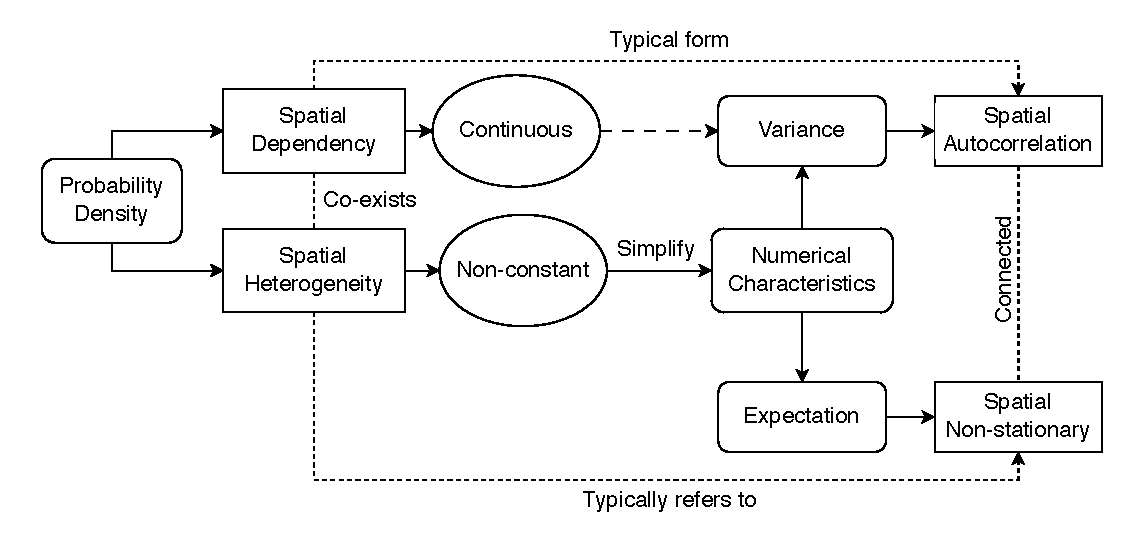
\includegraphics[width=\linewidth]{fig/spatial-dependence-heterogeneity.pdf}
  \caption{Relationships between spatial dependence, spatial heterogeneity, spatial non-stationarity, and spatial autocorrelation.}
  \label{fig:rel-spatial-depen-hetero}
\end{figure}

Furthermore, although both spatial autocorrelation and spatial non-stationarity reflect certain aspects (the variance and expectation, respectively) of spatial heterogeneity,
spatial autocorrelation is generally regarded as a manifestation of spatial dependence, whereas spatial non-stationarity is viewed as a form of spatial heterogeneity.
Therefore, the term ``spatial heterogeneity'' in the following discussion will refer solely to spatial non-stationarity,
aligning with the majority of studies that utilise geographically weighted regression \citep{HelbichBrunauer-2014,LuCharlton-2014,FotheringhamCrespo-2015,LuBrunsdon-2017,LuGe-2020a}.
Nonetheless, we propose viewing spatial heterogeneity and spatial dependence as broader, abstract properties that describe the conditional probability distribution of spatial random variables.
Correspondingly, spatial non-stationarity and spatial autocorrelation should be seen as more specific attributes, characterising the expectations and variances of spatial random variables, respectively.

\subsection{From the definition to the testing logic}\label{sec:heterogeneity-testing-logic}

The definitions above determine what needs to be tested.
The strong definition concerns the complete conditional density $f_{X|\vU}(x|\vu)$.
Testing equality of the complete density at all locations would be difficult in practice and is not necessary for the purpose of \gls{hgwr}, where the primary interest is whether a conditional relationship changes across space.
Therefore, we use the weak definition based on the conditional expectation.
Let $g(\vu)=E(X|\vU=\vu)$.
The absence of spatial non-stationarity means that $g(\vu)$ is constant for all possible locations, while spatial heterogeneity exists when at least one location has a different conditional expectation.

This statement gives the first part of the testing logic: a test of spatial heterogeneity is a test of spatial constancy, rather than a test of whether an effect is different from zero.
For the $k$-th \gls{glsw} effect in \gls{hgwr}, this definition leads to the null hypothesis
\begin{equation}\label{equ:glsw-heterogeneity-core-hypothesis}
  H_0: \gamma_{1k}=\gamma_{2k}=\cdots=\gamma_{mk},
\end{equation}
whereas the alternative hypothesis states that not all $\gamma_{jk}$ are equal.
An effect can therefore be significantly different from zero but spatially homogeneous, or spatially heterogeneous even when some local estimates are not significantly different from zero.

The second part of the logic is to measure departure from spatial constancy.
After estimating $\gamma_{jk}$ at all group locations, its spatial dispersion can be used as a statistic.
For the $k$-th \gls{glsw} effect, denote this statistic by
\begin{equation}\label{equ:heterogeneity-core-statistic}
  T_k = \frac{1}{m}\sum_{j=1}^{m}\left(\hat{\gamma}_{jk}-\overline{\hat{\gamma}}_k\right)^2,
\end{equation}
where $m$ is the number of groups and $\overline{\hat{\gamma}}_k$ is the mean of the local estimates.
A large value of $T_k$ indicates strong variation, but it cannot alone show significant spatial heterogeneity because random error, data borrowing, and the hierarchical random effects also produce variation in local estimates.

The final part is consequently to determine the distribution of a dispersion statistic under spatial constancy.
There are two routes in this study.
The bootstrap compares the observed variance of standardised local estimates with its empirical null distribution.
The distribution-based method uses the linear form of the \gls{glsw} estimator, the hat matrix $\vS$, and the covariance matrix $\vV$ to approximate the null distribution of an observation-weighted coefficient variance by an $F$ distribution.
The two methods address the same null hypothesis, but use different finite-sample statistics and reference distributions.
The following section incorporates the hierarchical error structure and \gls{glsw} estimator to construct the corresponding bootstrap and $F$ tests for \gls{hgwr}.

\section{Testing Spatial Heterogeneity in GLSW Effects} \label{sec:glsw-test}

According to \autoref{sec:heterogeneity-testing-logic}, testing a \gls{glsw} effect is to determine whether its variation among locations is significantly greater than the variation generated under a spatially constant effect.
The target is different from the conventional test of whether a coefficient is significantly different from zero.
For the $k$-th \gls{glsw} effect, both methods below evaluate the spatial constancy stated in \eqref{equ:glsw-heterogeneity-core-hypothesis}.
The bootstrap obtains an empirical reference distribution by repeated model fitting, while the distribution-based method derives an approximate $F$ distribution from the \gls{glsw} estimator.

% In this section, we concentrate on designing hypothesis tests for fixed effects and \gls{glsw} effects of the \gls{hgwr} model.
% The significance of deviation from zero is evaluated for both fixed effects and \gls{glsw} effects using a $t$-test.
% Additionally, testing spatial heterogeneity is considered for \gls{glsw} effects using an $F$-test and a bootstrap test.

% \subsection{Fixed effects}\label{sec:test-hgwr-fixed}

% For the $j$-th fixed effect, ${\beta}_j$, we test the following hypothesis as shown in \eqref{equ:hgwr-test-fixed-hypothesis},
% \begin{align}\label{equ:hgwr-test-fixed-hypothesis}
%     \begin{split}
%     H_0 &: {\beta}_j = 0 \; ; \\
%     H_1 &: {\beta}_j \neq 0 \; .
%     \end{split}
% \end{align}
% First, we obtain their variance as \eqref{equ:var-beta},
% \begin{equation} \label{equ:var-beta}
% \begin{split}
%     \var(\hat{\vbeta}) 
%     & = \left(\vX\T\vV^{-1}\vX\right)^{-1}\left(\vX\T\vV^{-1}\right) \var(\vy_h^{(t)}) 
%     \left[\left(\vX\T\vV^{-1}\vX\right)^{-1}\left(\vX\T\vV^{-1}\right)\right]\T \\
%     & = \left(\vX\T\vV^{-1}\vX\right)^{-1}\vX\T\vV^{-1}
%     \vV\vV^{-1}\vX \left[\left(\vX\T\vV^{-1}\vX\right)^{-1}\right]\T \\
%     & = \left(\vX\T\vV^{-1}\vX\right)^{-1} \; .
% \end{split}
% \end{equation}
% The test statistic used to evaluate the null hypothesis is \eqref{equ:hgwr-test-fixed-statistic}
% \begin{equation}\label{equ:hgwr-test-fixed-statistic}
%     t = \frac{\hat{\beta}_j}{\mathrm{se}(\hat{\beta}_j)} \sim t(\DF)
% \end{equation}
% where $\mathrm{se}(\hat{\beta}_j)$ is the squared root of the $j$-th diagonal element of 
% $\var(\hat{\vbeta})$, and $\DF$ is the degree of freedom of this model.

% For an \gls{hgwr} model with $p$ fixed effects, $q$ \gls{slr} effects, $r$ \gls{glsw} effects, $n$ observations, and $m$ groups, the total number of parameters is given by \eqref{equ:hgwr-test-np},
% \begin{equation}\label{equ:hgwr-test-np}
%     \NP = r m + p + \frac{q(q+1)}{2} + 1
% \end{equation}
% However, due to the data borrowing process, the \gls{glsw} effect parameters are not fully independent.
% Thus, we estimate the effective number of parameters of \gls{glsw} effects as \eqref{equ:hgwr-enp-glsw},
% \begin{equation}\label{equ:hgwr-enp-glsw}
%     \ENP_{\vgamma} = 2\tr(\vS) - \tr(\vS\T\vS)
% \end{equation}
% where
% \begin{equation*}
% \vS = \begin{pmatrix}
%     \mybm{g}_{1}(\mybm{G}^{\mathrm{T}}\mybm{W}_{1}\mybm{V}\mybm{G})^{-1}(\mybm{G}^{\mathrm{T}}\mybm{W}_{1}\mybm{V}\mybm{y}_{g}) \\
%     \mybm{g}_{1}(\mybm{G}^{\mathrm{T}}\mybm{W}_{1}\mybm{V}\mybm{G})^{-1}(\mybm{G}^{\mathrm{T}}\mybm{W}_{1}\mybm{V}\mybm{y}_{g})  \\
%     \vdots  \\
%     \mybm{g}_{1}(\mybm{G}^{\mathrm{T}}\mybm{W}_{1}\mybm{V}\mybm{G})^{-1}(\mybm{G}^{\mathrm{T}}\mybm{W}_{1}\mybm{V}\mybm{y}_{g}) \\
%     \vdots \\
%     \mybm{g}_{m}(\mybm{G}^{\mathrm{T}}\mybm{W}_{m}\mybm{V}\mybm{G})^{-1}(\mybm{G}^{\mathrm{T}}\mybm{W}_{m}\mybm{V}\mybm{y}_{g}) \\
%     \mybm{g}_{m}(\mybm{G}^{\mathrm{T}}\mybm{W}_{m}\mybm{V}\mybm{G})^{-1}(\mybm{G}^{\mathrm{T}}\mybm{W}_{m}\mybm{V}\mybm{y}_{g}) \\
%     \vdots \\
%     \mybm{g}_{m}(\mybm{G}^{\mathrm{T}}\mybm{W}_{m}\mybm{V}\mybm{G})^{-1}(\mybm{G}^{\mathrm{T}}\mybm{W}_{m}\mybm{V}\mybm{y}_{g})
% \end{pmatrix}
% \end{equation*}
% and $\vS$, known as the ``hat matrix'' \citep{FotheringhamBrunsdon-2002}, calculates the effective number of parameters and the effective degrees of freedom for the entire model as \eqref{equ:hgwr-enp} and \eqref{equ:hgwr-edf}, respectively,
% \begin{align}
% \label{equ:hgwr-enp}
% \ENP & = 2\tr(\vS) - \tr(\vS\T\vS) + p + \frac{q(q+1)}{2} + 1 \\
% \label{equ:hgwr-edf}
% \EDF & = n - \ENP \; .
% \end{align}

% \subsection{Group-level spatially weighted effects}\label{sec:test-hgwr-glsw}

\subsection{Bootstrap-based method}\label{sec:test-hgwr-glsw-boot}

The primary objective for the \gls{glsw} effects is to determine whether their spatial variation is significant under the definition and null hypothesis established in \autoref{sec:heterogeneity-testing-logic}.
The hypothesis is formulated as \eqref{equ:hgwr-glsw-boot-hypothesis},
\begin{align}\label{equ:hgwr-glsw-boot-hypothesis}
    \begin{split}
    H_0 &: \forall \vu, E(\hat{\vgamma}|\vu) = E(\hat{\vgamma}) \; ; \\
    H_1 &: \exists \vu, E(\hat{\vgamma}|\vu) \neq E(\hat{\vgamma}) \; .
    \end{split}
\end{align}
Because the \gls{glsw} effects are estimated within a hierarchical regression model, their local estimates inherit correlation from data borrowing and the model's error structure.
Both theoretical and experimental findings indicate that directly testing for spatial heterogeneity in \gls{glsw} effect estimates results in an excessively high Type I error rate (i.e., incorrectly rejecting the null hypothesis of no spatial heterogeneity), making the test ineffective.
For regression models, there are two typical resampling strategies: sampling observations and sampling residuals \citep{Bittmann-2021}.
For \gls{hgwr}, experiments show that resampling observations may lead to an insufficient number of samples in some locations, potentially causing model calibration to fail.
Therefore, resampling residuals is a more suitable approach, as recommended by \citet{HarrisBrunsdon-2017}.

For a calibrated \gls{hgwr} model with $\hat{\vgamma}$ as estimates of \gls{glsw} effects, $\hat{\vbeta}$ as estimates of fixed effects, and $\hat{\vD}$ as the estimated variance--covariance matrix of random effects, the distribution of the combined random-effect and residual term can be expressed as \eqref{equ:glsw-bootvar-error-distribution},
\begin{equation}\label{equ:glsw-bootvar-error-distribution}
    \ve = \vZ\vmu + \vepsilon \sim \vN\left(\vzero, (\vZ\vD\vZ\T+\vI)\sigma^2\right)
\end{equation}
The null model is fitted separately for each effect under test.
For effect $k$, that group-level variable is moved from the \gls{glsw} component to the fixed component, while the other \gls{glsw} effects retain their fitted spatial surfaces.
This imposes spatial constancy on the tested effect without imposing the same restriction on the remaining effects.
The observed coordinates, covariates, group membership, and group sample sizes are held fixed.
Bootstrap responses are generated from the fixed and \gls{glsw} components of this null model plus newly simulated zero-mean group random effects and residuals; empirical random-effect predictions are not included in the generating mean.
The procedure is as follows.
\begin{enumerate}[label=\textbf{Step \arabic*.}, left=0.5em, itemindent=2em]
    \item For the original model, calculate the variance of the standardised local estimates $\hat{\gamma}_{jk}/\widehat{\operatorname{se}}(\hat{\gamma}_{jk})$, denoted by $S_k$;
    \item Fit the effect-wise spatially constant null model and obtain its mean $\hat{\vy}_{0k}$, random-effect covariance $\hat{\vD}_{0k}$, and residual scale $\hat{\sigma}_{0k}$;
    \item Repeat the following steps $B$ times. In each iteration $i$,
    \begin{enumerate}
        \item Independently draw new group random effects and residuals according to \eqref{equ:glsw-bootvar-error-distribution}, using $\hat{\vD}_{0k}$ and $\hat{\sigma}_{0k}$, and set $\vy^*_i=\hat{\vy}_{0k}+\ve^*_i$;
        \item Refit the original \gls{hgwr} specification to $\vy^*_i$, normally holding the bandwidth at its value selected from the observed data;
        \item Calculate the standardised-variance statistic $S^*_{ik}$;
    \end{enumerate}
    \item Calculate the $p$ value as \eqref{equ:glsw-bootvar-pvalue},
    \begin{equation}\label{equ:glsw-bootvar-pvalue}
        p_k = \frac{1+\sum_{i=1}^B 1_{S^*_{ik} \geq S_k}}{B+1}
    \end{equation}
    and compare $p_k$ with the pre-defined significance level $\alpha$.
\end{enumerate}

Although \gls{hgwr} is more efficient than \gls{gwr} and \gls{mgwr} \citep{HuHarris-2024}, the entire procedure remains time-intensive.
We use $B=199$ in the primary Monte Carlo experiments and $B=999$ in a small diagnostic confirmation.
The historical fitted-model bootstrap is retained only as a diagnostic comparator; it is not used as the primary bootstrap procedure.

\subsection{Distribution-based method}\label{sec:test-hgwr-glsw-ftest}

As a computationally inexpensive approximation,
we can also design a probability-based hypothesis test for \gls{glsw} effects following the method proposed by \citet{LeungMei-2000}.
Assuming normality for $\vmu$ and $\vepsilon$,
we define the null and alternative hypothesis as \eqref{equ:hypothesis-glsw-ftest},
\begin{equation}\label{equ:hypothesis-glsw-ftest}
    \begin{split}
        H_{0} & : \gamma_{0k} = \gamma_{2k} = \cdots = \gamma_{mk}  \\
        H_{1} & : \mbox{not all $\gamma_{ik}(i=1,2,\cdots,m)$ are equal.}
    \end{split}
\end{equation}
For the $k$-th \gls{glsw} effect, we examine its variance under the null hypothesis, $V_k^2$, as \eqref{equ:glsw-ftest-variance},
\begin{equation}\label{equ:glsw-ftest-variance}
    \begin{split}
        V_{k}^2 & = \frac{1}{n} \sum_{i=1}^m \left( \hat{\gamma}_{ik} - \frac{1}{n} \sum_{i=1}^n \hat{\gamma}_{ik} \right)^2 = \frac{1}{n} \hat{\mybm{\gamma}}_{k}^{\mathrm{T}}\left( \mybm{I} - \frac{1}{n} \mybm{J} \right) \hat{\mybm{\gamma}}_{k} \\
        & =  \frac{1}{n} \left[ \hat{\mybm{\gamma}}_{k} - E(\hat{\mybm{\gamma}}_{k}) \right]^{\mathrm{T}} \left( \mybm{I} - \frac{1}{n} \mybm{J} \right)\left[ \hat{\mybm{\gamma}}_{k} - E(\hat{\mybm{\gamma}}_{k}) \right] \; .
    \end{split}
\end{equation}
According to \eqref{equ:bfml-glsw-estimator}, for the $i$-th group, we know
\begin{equation*}
    \hat{\mybm{\gamma}}_{ik} = \mybm{e}_{k} \left( \mybm{G}^{\mathrm{T}}\mybm{W}_{i}\mybm{V}^{-1}\mybm{G} \right)^{-1}\left( \mybm{G}^{\mathrm{T}}\mybm{W}_{i}\mybm{V}^{-1}\mybm{y}_{g} \right) = \mybm{\Gamma}_{i}\mybm{y}_{g}
\end{equation*}
where $\ve_k$ is the $(k+1)$-th row of the identity matrix $\vI$.
Let
\begin{equation}\label{equ:ftest-glsw-Gamma-full}
\mybm{\Gamma} = \begin{pmatrix}
\mybm{\Gamma}_{1}\T & \mybm{\Gamma}_{1}\T & \cdots & \mybm{\Gamma}_{1}\T & \cdots &
\mybm{\Gamma}_{m}\T & \mybm{\Gamma}_{m}\T & \cdots &
\mybm{\Gamma}_{m}\T
\end{pmatrix}\T
\end{equation}
where each $\vGamma_j$ represents $n_j$ times, with $n_j$ being the number of samples in the $j$-th group.
In this case, $E(\hat{\mybm{\gamma}_{k}})=\mybm{\Gamma}E(\mybm{y}_{g})$, and
\begin{equation*}
    V_{k}^2  = \mybm{\eta}^{\mathrm{T}}\left[ \frac{1}{n} \mybm{\Gamma}\left( \mybm{I}-\frac{1}{n} \mybm{J}\right)\mybm{\Gamma} \right]\mybm{\eta}
\end{equation*}
where $\mybm{\eta}=\mybm{Z}\mybm{\mu}+\mybm{\epsilon}\sim \mybm{N}(\mybm{0},\vV\sigma^2)$.
The expectation and variance of $V_k^2/\sigma^2$ can be calculated as \eqref{equ:glsw-ftest-exp-Vksigma} and \eqref{equ:glsw-ftest-var-Vksigma}, respectively,
\begin{align}
\label{equ:glsw-ftest-exp-Vksigma}
E\left( \frac{V_{k}^2}{\sigma^{2}} \right)  & = \mathrm{tr}\left[ \frac{1}{n} \mybm{\Gamma}^{\mathrm{T}} \left( \mybm{I}-\frac{1}{n}\mybm{J} \right) \mybm{\Gamma} \mybm{V} \right]  \\
\label{equ:glsw-ftest-var-Vksigma}
\mathop{\mathrm{var}}\left( \frac{V_{k}^2}{\sigma^{2}} \right) & = 2\mathrm{tr}\left\{ \left[ \frac{1}{n} \mybm{\Gamma}^{\mathrm{T}} \left( \mybm{I}-\frac{1}{n}\mybm{J} \right) \mybm{\Gamma}\mybm{V} \right]^2 \right\} .
\end{align}
The matrix square in \eqref{equ:glsw-ftest-var-Vksigma} is evaluated before taking the trace, so the second-order moment includes cross-location as well as within-location covariance terms.
By letting $\xi_{1}=E({V_{k}^2}/{\sigma^2})$ and $\xi_{2}=\frac{1}{2}\mathop{\mathrm{var}}({V_{k}^2}/{\sigma^2})$,
the term $\hfrac{\xi_{1}V_{k}^2}{\xi_{2}\sigma^2}$ can be approximated by a $\chi^2$ distribution with $\hfrac{\xi_1^2}{\xi_2}$ degrees of freedom.

Denote the sum of squared residuals of $\hat{\vy}_g$ by $\mathrm{RSS}_g$ as \eqref{equ:glsw-ftest-rss},
\begin{equation}\label{equ:glsw-ftest-rss}
    \begin{split}
    \mathrm{RSS}_{g} & = \mybm{y}_{g}^{\mathrm{T}}(\mybm{I}-\mybm{S})^{\mathrm{T}}(\mybm{I}-\mybm{S})\mybm{y}_{g} = \mybm{\eta}^{\mathrm{T}}(\mybm{I}-\mybm{S})^{\mathrm{T}}(\mybm{I}-\mybm{S})\mybm{\eta} \quad .
    \end{split}
\end{equation}
where $\vS$ is defined in \eqref{equ:bfml-glsw-hatmat}.
Using a similar method as above, the expectation and variance of $\left.\mathrm{RSS}\middle/\sigma^2\right.$ can be calculated as \eqref{equ:glsw-ftest-rsssigma2-exp} and \eqref{equ:glsw-ftest-rsssigma2-var},
\begin{align}
\label{equ:glsw-ftest-rsssigma2-exp}
E\left( \frac{\mathrm{RSS}_{g}}{\sigma^{2}} \right) & = \mathrm{tr}\left[ (\mybm{I}-\mybm{S})^{\mathrm{T}}(\mybm{I}-\mybm{S})\mybm{V} \right]  \\
\label{equ:glsw-ftest-rsssigma2-var}
\mathop{\mathrm{var}}\left( \frac{\mathrm{RSS}_{g}}{\sigma^{2}} \right) & = 2\mathrm{tr}\left\{ \left[ (\mybm{I}-\mybm{S})^{\mathrm{T}}(\mybm{I}-\mybm{S})\mybm{V} \right]^2 \right\} \quad .
\end{align}
By setting $\delta_{1}=E\left( \frac{\mathrm{RSS}_{g}}{\sigma^{2}} \right)$ and 
$\delta_{2}=\frac{1}{2}\mathop{\mathrm{var}}\left( \frac{\mathrm{RSS}_{g}}{\sigma^{2}} \right)$,
the term $\frac{\delta_1\mathrm{RSS}_g}{\delta_2\sigma^2}$ can be approximated by a $\chi^2$ distribution with $\delta_1^2/\delta_2$ degrees of freedom.
Furthermore, since $\hat{\sigma}^2 = \frac{\mathrm{RSS}_g}{\delta_1}$
is an unbiased estimator of $\sigma^2$, $\frac{\delta_1\mathrm{RSS}_g}{\delta_2\sigma^2}$ can be approximated by a $\chi^2$ distribution according to \eqref{equ:glsw-ftest-rss-chi2},
\begin{equation}\label{equ:glsw-ftest-rss-chi2}
    \frac{\delta_1\mathrm{RSS}_g}{\delta_2\sigma^2} = \frac{\delta_1^2 \hat{\sigma}^2}{\delta_2\sigma^2} \sim \chi^2\left(\frac{\delta_1^2}{\delta_2}\right).
\end{equation}

Consequently, we can design an $F$-statistic as \eqref{equ:glsw-ftest-statistics},
\begin{equation}\label{equ:glsw-ftest-statistics}
F = \frac{
\left( \frac{\xi_{1}V_{k}^{2}}{\xi_{2}\sigma^{2}} \middle/ \frac{\xi_{1}^{2}}{\xi_{2}} \right) 
}{
\left( \frac{\delta_{1}^{2}\hat{\sigma}^{2}}{\delta_{2}\sigma^{2}} \middle/ \frac{\delta_{1}^{2}}{\delta_{2}} \right) 
} = \frac{V_{k}^{2}}{\xi_{1}\hat{\sigma}^{2}} \sim F\left( \frac{\xi_{1}^{2}}{\xi_{2}} , \frac{\delta_{1}^{2}}{\delta_{2}} \right)
\end{equation}
For significance level $\alpha$, let $F_{1-\alpha}$ denote the corresponding upper critical quantile.
We reject the null hypothesis if $F \geqslant F_{1-\alpha}$.

% \subsection{Sample-level random effects}

% Like the \gls{glsw} effects, an important question in testing the significance of \gls{slr} effects is whether they are heterogeneous between groups instead of whether they are significantly different from zero.
% For \gls{slr} effects, which are similar to the random effects in \gls{hlm}, we use the likelihood ratio test typically \citep{MyersMontgomery-2012}.
% For a full model and a reduced model, their log-likelihood functions have values $l^{\mathrm{Full}}$ and $l^{\mathrm{Red}}$, respectively.
% The likelihood-ratio-test statistic is
% \begin{equation}
%     \hat{\lambda} = -2 l^{\mathrm{Full}} + 2 l^{\mathrm{Red}} \; .
% \end{equation}
% Test by removing one random effect each time is suggested.
% In this case, the $p$-value is calculated by
% \begin{equation}
%     p = \frac{1}{2} P\left(\chi^2_{k} > \hat{\lambda}\right) +
%     \frac{1}{2} P\left(\chi^2_{k-1} > \hat{\lambda}\right)
% \end{equation}
% where $k$ is the number of random effects (including the random intercept) in the full model.

\subsection{Simulation}\label{sec:test-hgwr-simulation}

The Monte Carlo experiment uses 200 group locations drawn independently and uniformly from $[0,1]\times[0,1]$ with a fixed coordinate seed.
The same locations are retained across scenarios and repetitions so that differences among rejection rates do not reflect a changing spatial configuration.
For each simulated data set, group sizes are independently sampled from the discrete uniform distribution on 20--50, and the group-level covariates $g_1$ and $g_2$ and sample-level covariates $x_1,x_2,x_3,z_1$ are generated independently from standard normal variables.
The group-level covariates have no imposed spatial autocorrelation, mutual correlation, or correlation with a latent spatial process.

Let $s(u_j)$ be the standardised value across the 200 locations of
\begin{equation}\label{equ:sim-hgwrtest-surface}
  \frac{1}{324}\left[36-\left(6-\frac{12u_j}{2}\right)^2\right]^2.
\end{equation}
The two \gls{glsw} effects are $\gamma_{1j}=2+a s(u_j)$ and $\gamma_{2j}=2$, where $a\in\{0,0.5,1\}$ controls the heterogeneity of the first effect.
Responses are generated as
\begin{equation}\label{equ:sim-hgwrtest-response}
  y_{ij}=2+g_{1j}\gamma_{1j}+g_{2j}\gamma_{2j}+2x_{1ij}+b_{0j}+b_{1j}z_{1ij}+\epsilon_{ij},
\end{equation}
where $b_{0j}\sim N(0,\tau^2)$, $b_{1j}\sim N(2,0.2^2)$, and $\epsilon_{ij}\sim N(0,1)$ in the core experiment.
We set $\tau^2=\mathrm{ICC}/(1-\mathrm{ICC})$ for ICC values 0.1 and 0.4; ICC here labels the random-intercept variance setting rather than the complete marginal correlation induced by the random slope.
Each data set is fitted as
\begin{equation}\label{equ:simulation-fitted-model}
  y_{ij}=\gamma_{1j}g_{1j}+\gamma_{2j}g_{2j}+\vbeta\T\vx_{ij}+b_{0j}+b_{1j}z_{1ij}+\epsilon_{ij}.
\end{equation}

The approximate $F$ test is evaluated in all six $a$-by-ICC scenarios using 500 independent data sets per scenario.
The effect-wise bootstrap uses $B=199$ resamples for 250 data sets under each global-null scenario and for 100 data sets at $a=0.5$ and $a=1$ with ICC 0.4.
The same simulated data sets and seeds are used when two methods are compared within a scenario.
The legacy fitted-model bootstrap is retained at the two ICC 0.4 endpoints using 50 data sets, and independent $B=999$ confirmation experiments use 20 data sets at each endpoint.
Two robustness scenarios replace the normal residuals by variance-standardised $t_5$ residuals or use strongly unbalanced group sizes.
They use 200 data sets for the $F$ test and 30 for the effect-wise bootstrap at $a=0.5$ and ICC 0.4.
A separate ten-data-set diagnostic re-selects the bandwidth within every bootstrap fit.
All tests use a 5\% threshold; rejection rates exclude non-converged fits, whose frequency is reported separately, and Wilson intervals quantify Monte Carlo uncertainty.

\begin{table*}[tbp]
  \centering\scriptsize
  \caption{Core and confirmation Monte Carlo results at the 5\% level. Each effect column gives usable/planned outer data sets followed by the rejection rate in per cent and its Wilson 95\% confidence interval. When $a>0$, $\gamma_1$ is heterogeneous and $\gamma_2$ remains spatially constant. Full-model denotes the existing \texttt{legacy}/\texttt{fitted} software mode; it samples around the fitted unrestricted model and is therefore a model-based reference rather than an effect-wise null test.}
  \label{tab:simulation-core-results}
  \resizebox{\textwidth}{!}{%
  \begin{tabular}{lrrrlllll}
    \toprule
    Procedure & $B$ & $a$ & ICC & $\gamma_1$: usable/planned & $\gamma_1$: rate (95\% CI) & $\gamma_2$: usable/planned & $\gamma_2$: rate (95\% CI) & Role \\
    \midrule
Effect-wise bootstrap & 199 & 0.0 & 0.1 & 244/250 & 3.7 (2.0--6.9) & 244/250 & 1.6 (0.6--4.1) & Primary \\
Effect-wise bootstrap & 199 & 0.0 & 0.4 & 248/250 & 3.2 (1.6--6.2) & 248/250 & 3.2 (1.6--6.2) & Primary \\
Effect-wise bootstrap & 199 & 0.5 & 0.4 & 98/100 & 96.9 (91.4--99.0) & 98/100 & 4.1 (1.6--10.0) & Primary \\
Effect-wise bootstrap & 199 & 1.0 & 0.4 & 98/100 & 100.0 (96.2--100.0) & 98/100 & 3.1 (1.0--8.6) & Primary \\
Full-model bootstrap & 199 & 0.0 & 0.1 & 248/250 & 0.0 (0.0--1.5) & 248/250 & 0.0 (0.0--1.5) & Model-based reference \\
Full-model bootstrap & 199 & 0.0 & 0.4 & 250/250 & 0.0 (0.0--1.5) & 250/250 & 0.0 (0.0--1.5) & Model-based reference \\
Full-model bootstrap & 199 & 0.5 & 0.1 & 100/100 & 1.0 (0.2--5.4) & 100/100 & 0.0 (0.0--3.7) & Model-based reference \\
Full-model bootstrap & 199 & 0.5 & 0.4 & 100/100 & 22.0 (15.0--31.1) & 100/100 & 0.0 (0.0--3.7) & Model-based reference \\
Full-model bootstrap & 199 & 1.0 & 0.1 & 100/100 & 0.0 (0.0--3.7) & 100/100 & 0.0 (0.0--3.7) & Model-based reference \\
Full-model bootstrap & 199 & 1.0 & 0.4 & 98/100 & 13.3 (7.9--21.4) & 98/100 & 0.0 (0.0--3.8) & Model-based reference \\
Approximate $F$ & -- & 0.0 & 0.1 & 498/500 & 9.4 (7.2--12.3) & 498/500 & 8.0 (6.0--10.8) & Primary \\
Approximate $F$ & -- & 0.0 & 0.4 & 500/500 & 6.0 (4.2--8.4) & 500/500 & 7.8 (5.8--10.5) & Primary \\
Approximate $F$ & -- & 0.5 & 0.1 & 495/500 & 100.0 (99.2--100.0) & 495/500 & 20.8 (17.5--24.6) & Primary \\
Approximate $F$ & -- & 0.5 & 0.4 & 499/500 & 100.0 (99.2--100.0) & 499/500 & 11.2 (8.7--14.3) & Primary \\
Approximate $F$ & -- & 1.0 & 0.1 & 499/500 & 100.0 (99.2--100.0) & 499/500 & 49.5 (45.1--53.9) & Primary \\
Approximate $F$ & -- & 1.0 & 0.4 & 497/500 & 100.0 (99.2--100.0) & 497/500 & 17.1 (14.0--20.7) & Primary \\
Effect-wise bootstrap (confirmation) & 999 & 0.0 & 0.4 & 20/20 & 5.0 (0.9--23.6) & 20/20 & 0.0 (0.0--16.1) & Confirmation \\
Effect-wise bootstrap (confirmation) & 999 & 1.0 & 0.4 & 20/20 & 100.0 (83.9--100.0) & 20/20 & 0.0 (0.0--16.1) & Confirmation \\
    \bottomrule
  \end{tabular}
  }
\end{table*}


Under the global null, the effect-wise bootstrap rejection rates range from 1.6\% to 3.7\%.
The 95\% intervals include 5\% except for $\gamma_2$ at ICC 0.1, where the method is conservative (1.6\%, 95\% CI 0.6--4.1\%).
At ICC 0.4, the bootstrap detects the heterogeneous $\gamma_1$ in 96.9\% of usable repetitions for $a=0.5$ and 100\% for $a=1$.
Over the same repetitions it rejects the constant $\gamma_2$ in only 4.1\% and 3.1\%, respectively.
This combination of detection and embedded-null behaviour supports the effect-wise bootstrap as the primary inferential procedure in the simulated settings.

The corrected $F$ approximation is less well calibrated.
Its global-null rejection rates range from 6.0\% to 9.4\%, with three of four effect-by-ICC estimates above 7\%.
Although it detects $\gamma_1$ in all usable heterogeneous repetitions, its rejection rate for the constant $\gamma_2$ increases with the heterogeneity of $\gamma_1$.
For $a=0.5$, these false-positive rates are 20.8\% at ICC 0.1 and 11.2\% at ICC 0.4; for $a=1$, they rise to 49.5\% and 17.1\%.
The apparent 100\% power of the $F$ test therefore cannot be interpreted independently of its loss of effect specificity.
The method remains useful as a rapid approximation, but the Monte Carlo results do not support treating it as a calibrated substitute or cross-validation for the effect-wise bootstrap.

The additional experiments are reported in the supplemental material.
The legacy bootstrap has no rejections under its 50-data-set null scenario but detects $\gamma_1$ in only 14.3\% of 49 usable strong-alternative repetitions.
The independent $B=999$ confirmation is directionally consistent with the primary effect-wise results, although 20 repetitions per endpoint yield wide confidence intervals.
Under $t_5$ residuals and strongly unbalanced group sizes, the effect-wise bootstrap detects $\gamma_1$ in 29 of 30 repetitions and does not reject $\gamma_2$; the corresponding zero-rejection intervals nevertheless have upper bounds of 11.4\%.
The bandwidth-reselection diagnostic succeeds for only one of ten data sets and provides no interpretable inferential result.

Across 4,310 outer repetitions, 35 (0.81\%) fail to produce usable tests.
For fixed-bandwidth experiments, the failure rates are 0.38\% for the $F$ test, 1.00\% for the legacy bootstrap, and 1.50\% for the effect-wise bootstrap.
All initial covariance optimisations report convergence and all usable estimates of $\vD$ are positive definite, indicating that the remaining failures arise principally from outer backfitting or bootstrap-refit iteration limits.
The median serial elapsed times are 1.44 seconds for the $F$ test, 73.92 seconds for the legacy bootstrap, and 132.67 seconds for the effect-wise bootstrap.

The simulation is conditional on one fixed spatial configuration and excludes spatially autocorrelated or spatially confounded covariates.
It also generates $b_{1j}$ with mean 2 while the fitted random-effect component is centred at zero without a separate fixed $z_1$ term.
The results consequently describe the implemented data-generating and fitting configuration, not calibration under every correctly specified \gls{hgwr} design.
\section{Case study: spatial inequalities in extracurricular education investment in China}\label{sec:qoe-case}

The simulations evaluate how the proposed procedures behave under known data-generating structures.
This section examines their role in an applied \gls{hgwr} analysis, where the assignment of a coefficient to the \gls{glsw} or fixed component affects both model complexity and substantive interpretation.
We study family expenditure on children's extracurricular courses in China.
The case is methodologically relevant because the outcome is observed for children and families, whereas several candidate explanations describe the provinces in which those families live.

\subsection{Context, data, and outcome}\label{sec:qoe-data}

Quality-oriented education, also known as \textit{suzhi jiaoyu}, was introduced as a national educational development strategy in 1993 \citep{CCCPC-1993}.
It seeks to foster development beyond examination performance, including aesthetic appreciation, physical education, and practical skills \citep{Dello-Iacovo-2009,LiuLi-2020-en}.
Extracurricular courses have become an important means of obtaining these forms of education \citep{ZhangTang-2017,ZhengYuan-2021}, but access is voluntary and largely market-mediated.
Consequently, participation and expenditure are related to household resources and parental choices \citep{ChiQian-2016,QianChi-2015-en,SongZhou-2019}, while the supply and price of courses also reflect regional economic development, public education investment, and urban--rural differences \citep{HuangGao-2017,XiangStillwell-2020,SuYuan-2023}.
These multiple levels make the application suitable for \gls{hgwr}, but they also make it important to distinguish a genuinely spatially heterogeneous provincial association from an estimated surface that varies only because of sampling uncertainty.

We combine four data sources.
The China Institute for Educational Finance Research Household Surveys (CIEFR-HS) collected family and child information from 40,011 families in 29 provincial-level administrations in 2017 and 34,643 families in 2019 \citep{CIEFR-HS,CIEFR-HS-V1,CIEFR-HS-2019}.
The surveys include household finances, parental education, child characteristics, education expenditure, and participation in extracurricular training.
Provincial economic and educational indicators are drawn from the \textit{China Statistical Yearbook} and the \textit{Educational Statistical Yearbook of China} \citep{KangSheng-2024,ESYC-2022}.
Provincial boundaries provide the locations used by the spatial weights, and 2017 point-of-interest data from Amap provide counts of youth palaces, institutions that supply extracurricular educational resources \citep{Lei-2024,LaiXu-2023}.
The study covers the 29 provinces identified in \autoref{fig:qoe-provinces}; the complete survey sample counts describe the source surveys rather than the final complete-case estimation sample.

\begin{figure}[tbp]
  \centering
  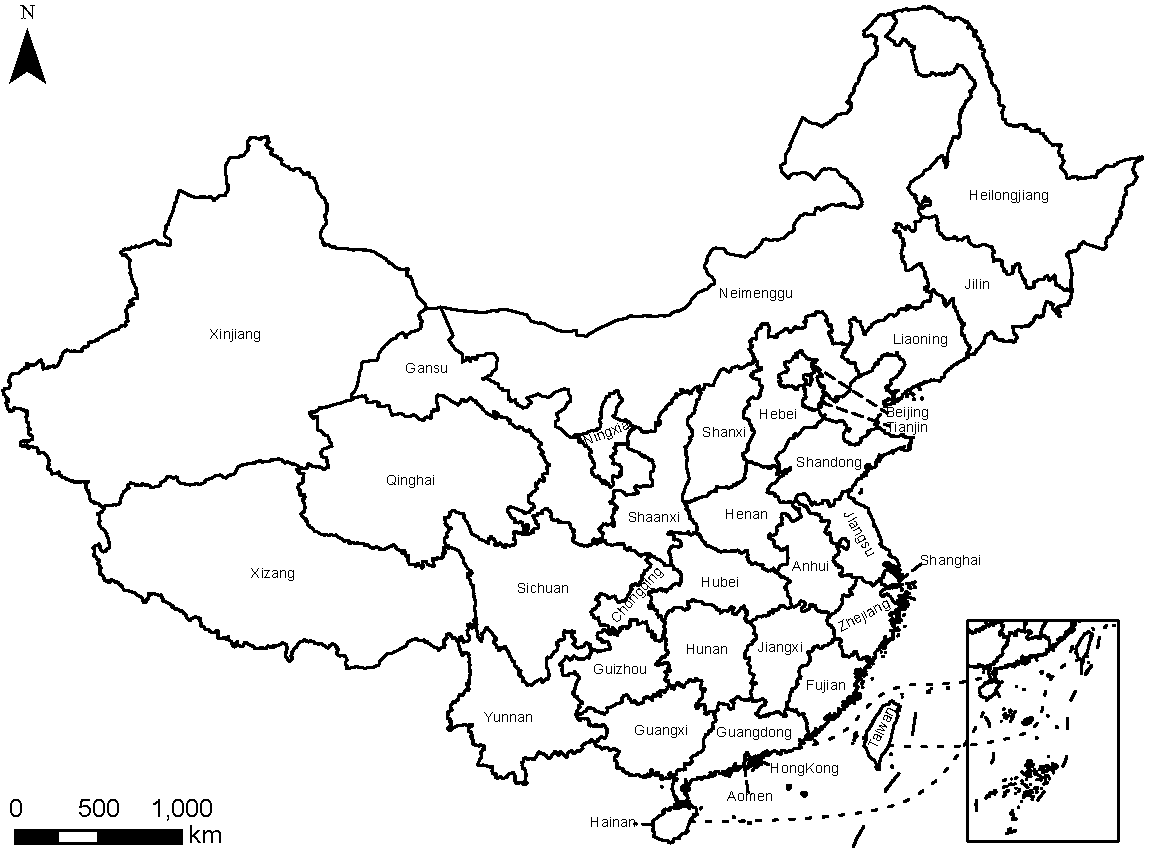
\includegraphics[width=0.82\linewidth]{fig/fig_ChinaProvinces.pdf}
  \caption{Provincial-level administrations covered by the CIEFR-HS data. The South China Sea Islands and national boundary shown in the inset lie outside the study area analysed here.}
  \label{fig:qoe-provinces}
\end{figure}

The main response, \QOESpendingPH, is the estimated hourly expenditure on extracurricular courses for one child.
Hourly expenditure is used as a proxy for the level of course resources purchased by a family, while recognising that price is an imperfect measure of educational quality.
An alternative model uses \QOESpendRatio, the ratio of extracurricular-course expenditure to total expenditure for the child, to describe the relative priority assigned to these courses.
The province-level covariates describe the primary-sector economy, living costs, income inequality, university recruitment, public education budgets, and the prevalence of highly educated residents.
The household-level covariates describe income, spending, assets, debt, parental education, the child's gender and age, and urban residence.

\subsection{Effect specification guided by heterogeneity tests}\label{sec:qoe-specification}

The case study uses the three-effect structure in \autoref{sec:hgwr}.
Province-level covariates are candidates for \gls{glsw} effects because their associations with family expenditure may vary geographically.
Household covariates are assigned fixed effects unless the grouped data support a sample-level random effect.
All continuous variables indicated in \autoref{tab:qoe-variables} are transformed and scaled as in the original QOE analysis.

\begin{table}[tbp]
  \centering\scriptsize
  \caption{Variables and effect types in the main QOE HGWR model. ``Log'' and ``Scale'' indicate the transformations used before estimation.}
  \label{tab:qoe-variables}
  \begin{tabular}{llll|llll}
    \toprule
    Variable & Effect & Log & Scale & Variable & Effect & Log & Scale \\
    \midrule
    \QOESpendingPH          & Response & Yes & Yes & \NumEnterprise          & Fixed & Yes & Yes \\
    \GDPPrimary             & \gls{glsw} & Yes & Yes & \CultCentCountTotal     & Fixed & Yes & Yes \\
    \Engel                  & \gls{glsw} & Yes & Yes & \TotalIncome            & Fixed & Yes & Yes \\
    \CPI                    & \gls{glsw} & Yes & Yes & \TotalSpending          & Fixed & Yes & Yes \\
    \Gini                   & \gls{glsw} & Yes & Yes & \Asset                  & Fixed & Yes & Yes \\
    \UniversityRecruitRatio & \gls{glsw} & Yes & No  & \Debt                   & Fixed & Yes & Yes \\
    \GeneralEduBudget       & \gls{glsw} & Yes & Yes & \Age                    & Fixed & Yes & Yes \\
    \HighEducated           & \gls{glsw} & Yes & Yes & \HighEdu                & Fixed & No  & No  \\
    \RegionUrban            & \gls{slr}  & No  & No  & \GenderMale             & Fixed & No  & No  \\
    \bottomrule
  \end{tabular}
\end{table}

The specification is not based on the visual variability of coefficient maps alone.
The original specification procedure first fits the remaining province-level variables as \gls{glsw} effects and uses the approximate $F$ test in \autoref{sec:test-hgwr-glsw-ftest} to screen each surface.
The youth-palace count is not rejected by this screening test and is therefore retained as a fixed rather than a \gls{glsw} effect.
This decision illustrates the inferential distinction motivating the paper: a variable may be substantively relevant or have a non-zero global association without requiring a geographically varying coefficient.
We also address clear multicollinearity between \GDPPrimary and \NumEnterprise by assigning the latter a fixed effect, and exclude national fiscal education expenditure because of its high correlation with \GeneralEduBudget.
Finally, an \gls{hlm} with forward selection identifies \RegionUrban as an \gls{slr} effect.
The resulting specification is shown in \autoref{tab:qoe-variables}.

\subsection{Evidence of spatial heterogeneity}\label{sec:qoe-heterogeneity-results}

\autoref{tab:qoe-model-summary} reports the main model.
The $F$ column gives the approximate test of whether each \gls{glsw} effect is spatially homogeneous across the study area; the percentages describe how many province-specific estimates reach each local significance level.
These are distinct inferential statements.
For example, an effect surface may be heterogeneous overall even when many individual provincial estimates are imprecise.
All retained \gls{glsw} effects reject spatial homogeneity according to the approximate $F$ test at the 5\% level, although the evidence is weaker for \Gini than for most other provincial variables.
The Monte Carlo experiment shows that this approximation can be liberal and can reject a constant effect when another \gls{glsw} effect is heterogeneous.
The case-study results are therefore treated as screening evidence rather than independent confirmation by a well-calibrated effect-wise test.

\begin{table}[tbp]
  \centering\scriptsize
  \caption{Summary of the main QOE HGWR model. For GLSW effects, the $F$ statistic is the approximate spatial-homogeneity test; percentages are the proportions of province-specific estimates in each significance category.}
  \label{tab:qoe-model-summary}
  \begin{tabular}{lrrrrrrr}
    \toprule
    GLSW & $\overline{\mathrm{Est.}}$ & $\overline{\mathrm{S.E.}}$ & $F$ & *** & ** & * & . \\
    \midrule
    \Intercept              &  5.939 & 3.534 & 3.562*** & 20.7\% & 20.7\% & 13.8\% &  0.0\% \\
    \GDPPrimary             &  1.797 & 1.164 & 4.206*** & 20.7\% & 13.8\% &  6.9\% &  3.4\% \\
    \Engel                  &  0.359 & 0.453 & 5.348*** &  0.0\% & 27.6\% & 17.2\% &  0.0\% \\
    \CPI                    & -0.424 & 0.596 & 6.765*** & 10.3\% & 10.3\% &  0.0\% &  3.4\% \\
    \Gini                   & -0.549 & 0.578 & 1.820*   &  0.0\% &  3.4\% & 17.2\% & 13.8\% \\
    \UniversityRecruitRatio & -0.478 &11.045 & 3.985*** &  0.0\% &  3.4\% & 20.7\% & 10.3\% \\
    \GeneralEduBudget       &  3.413 & 1.053 & 5.121*** & 44.8\% & 13.8\% & 13.8\% &  3.4\% \\
    \HighEducated           &  1.665 & 1.695 & 2.875**  &  3.4\% &  6.9\% & 13.8\% &  0.0\% \\
    \bottomrule
    \toprule
    Fixed & Est. & S.E. & $t$ & \multicolumn{2}{l}{SLR} & Mean & S.E. \\
    \cmidrule(r){1-4}\cmidrule(l){5-8}
    \Intercept          & -4.388 & 0.224 & 19.555*** & \multicolumn{2}{l}{\Intercept}   & 0.000 & 0.969 \\
    \NumEnterprise      & -4.323 & 0.557 &  7.759*** & \multicolumn{2}{l}{\RegionUrban} & 0.000 & 0.969 \\
    \CultCentCountTotal & -0.646 & 0.605 &  1.068    & & & & \\
    \TotalIncome        &  0.014 & 0.021 &  0.653    & & & & \\
    \TotalSpending      &  0.143 & 0.025 &  5.780*** & & & & \\
    \Asset              &  0.084 & 0.027 &  3.095**  & & & & \\
    \Debt               &  0.025 & 0.021 &  1.187    & & & & \\
    \HighEdu            &  0.281 & 0.049 &  5.775*** & & & & \\
    \GenderMale         & -0.101 & 0.041 &  2.448*   & & & & \\
    \Age                & -0.141 & 0.021 &  6.730*** & & & & \\
    \RegionUrban        &  0.473 & 0.214 &  2.211*   & & & & \\
    \bottomrule
    \multicolumn{8}{l}{Significance levels: . $p<0.1$, * $p<0.05$, ** $p<0.01$, *** $p<0.001$.}
  \end{tabular}
\end{table}

\begin{figure}[tbp]
  \centering
  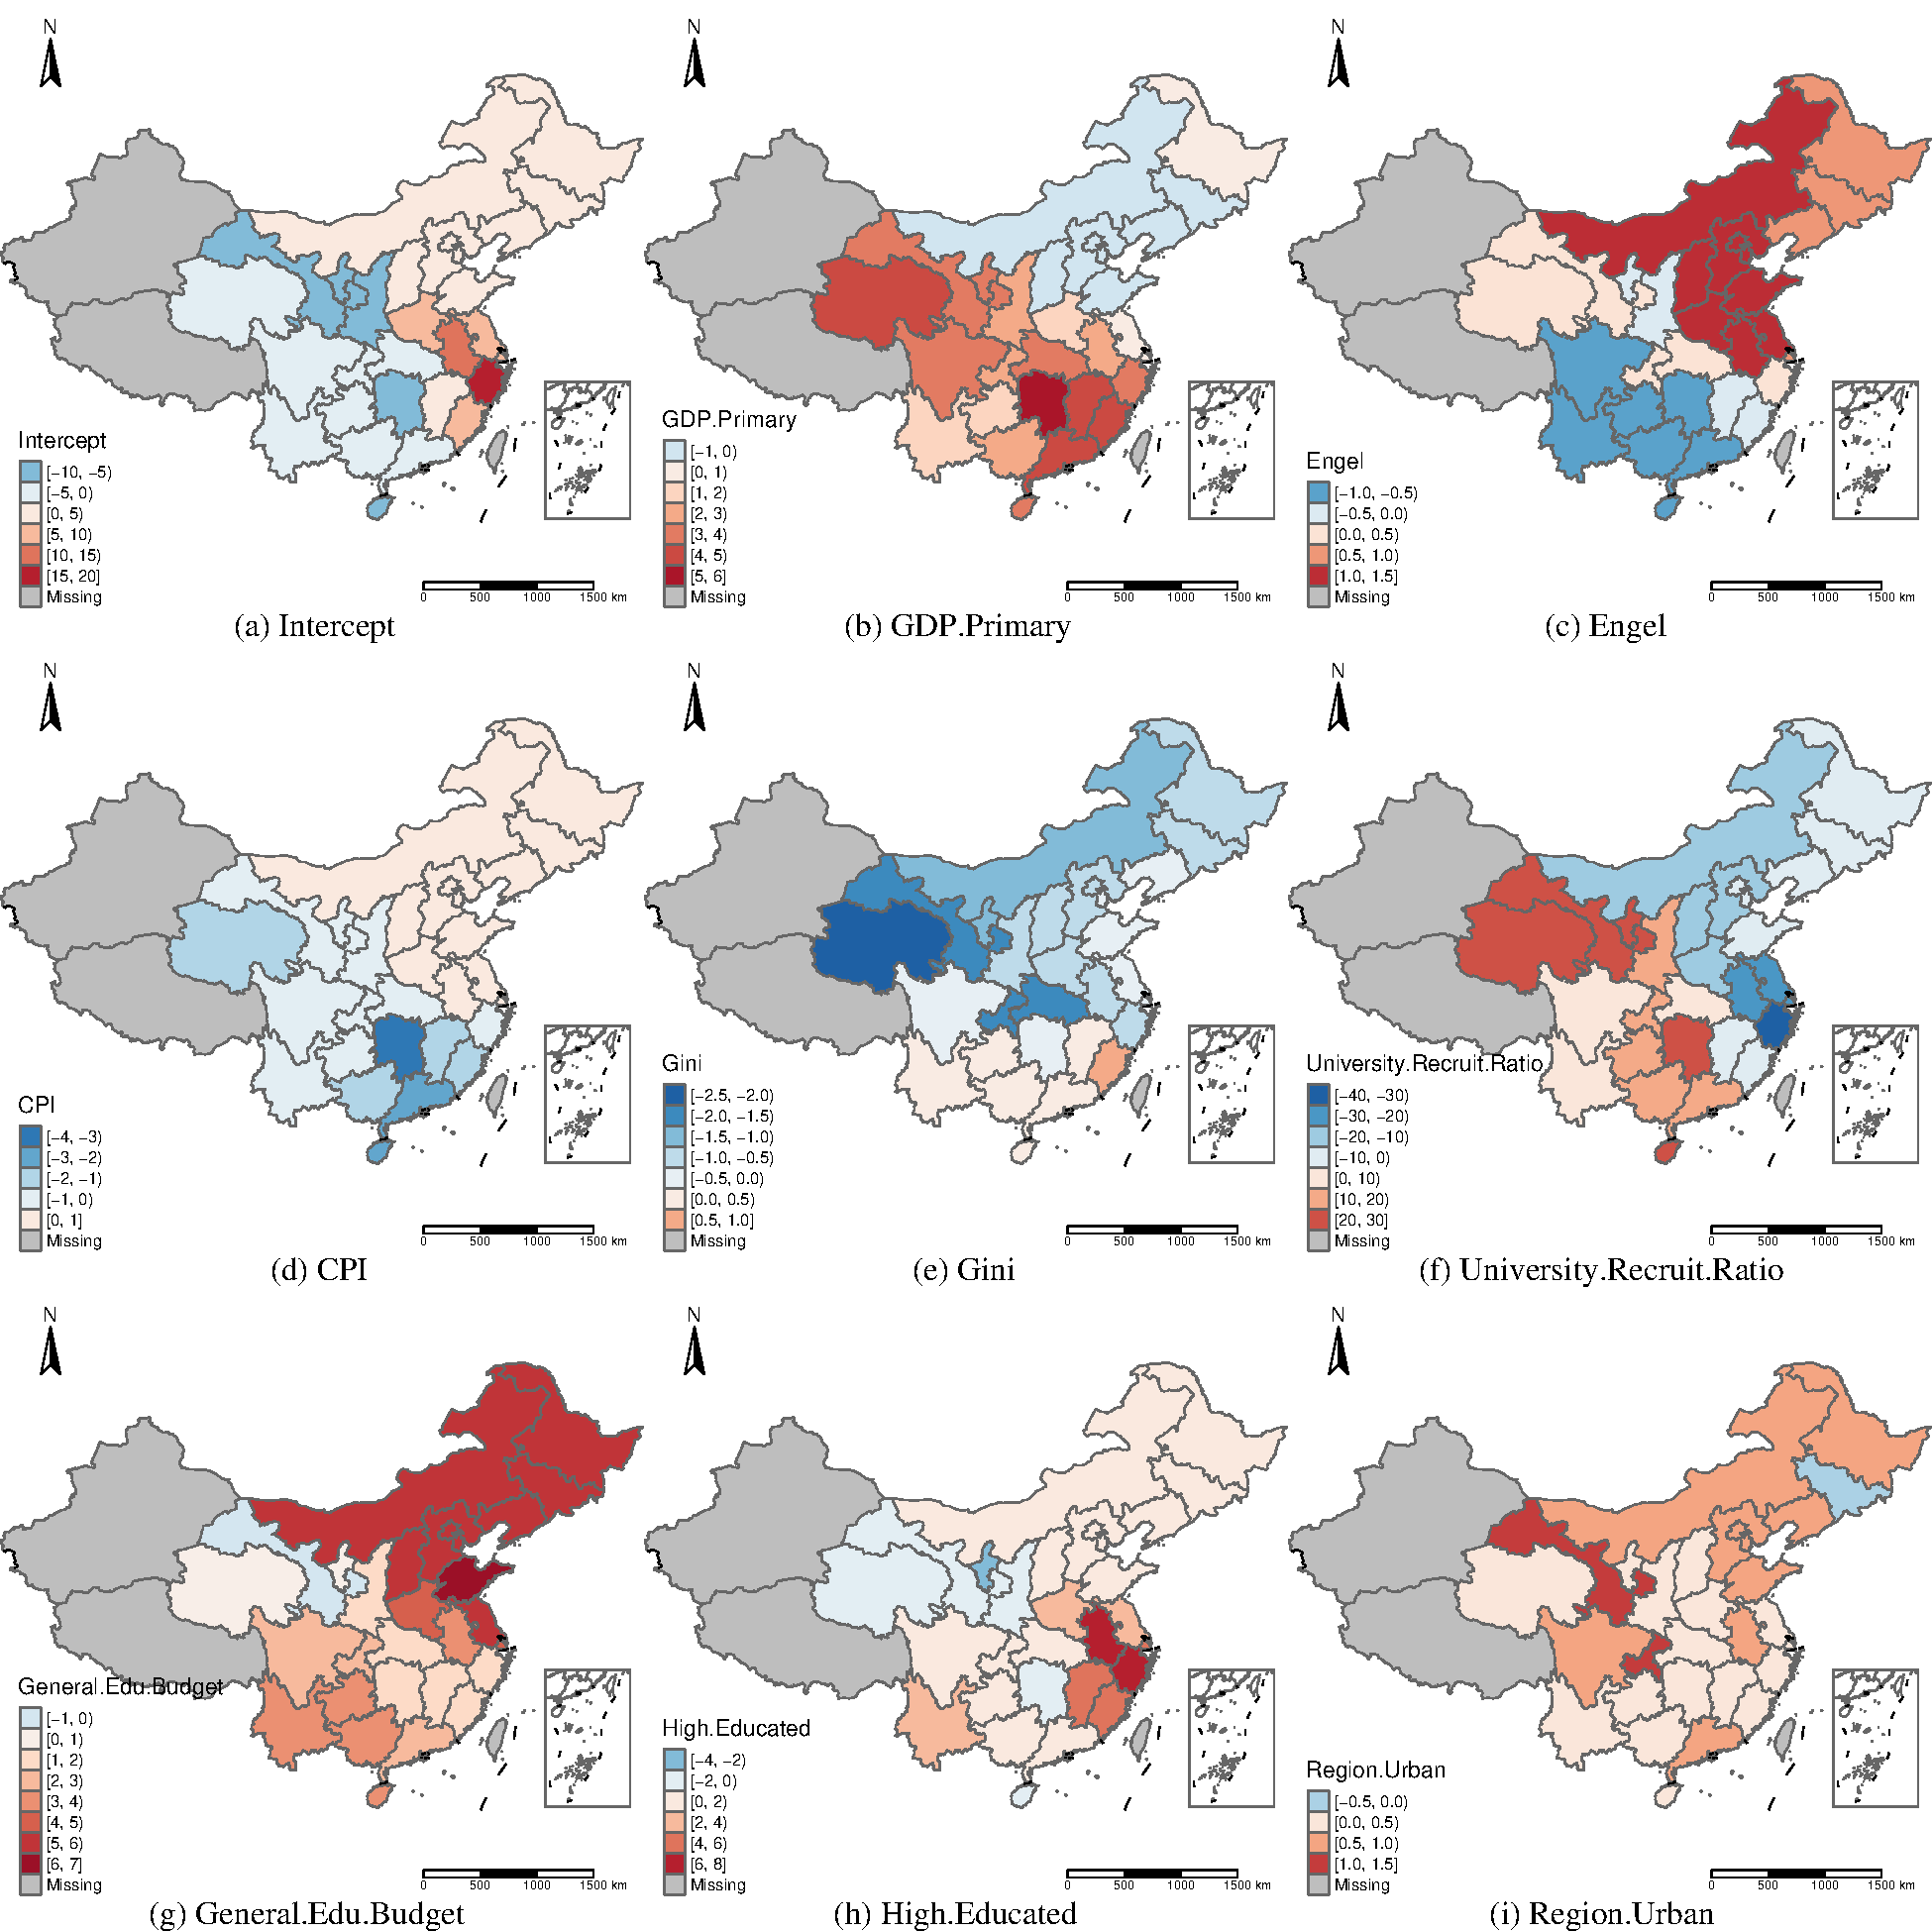
\includegraphics[width=\linewidth]{fig/fig_Model19_coef.pdf}
  \caption{Province-specific estimates of the GLSW effects and the SLR effect for urban residence in the main QOE model. The approximate global $F$ results in \autoref{tab:qoe-model-summary} provide screening evidence against spatial homogeneity; visual variation alone is not a test.}
  \label{fig:qoe-coefficients}
\end{figure}

The estimated surfaces in \autoref{fig:qoe-coefficients} show that different provincial factors have different geographies.
The association of primary-sector GDP with hourly expenditure is positive and locally significant in parts of central, southern, and western China, consistent with the possibility that agricultural development raises the resources available to some rural households.
The consumer price index has negative and locally significant estimates in parts of southern China, including Hunan, Guangdong, and Hainan, although living costs could affect both household purchasing power and course prices.
The Gini coefficient is negative in several central, northern, and western provinces, but many provincial estimates are not significant; its global heterogeneity test should therefore not be read as evidence of a negative association everywhere.

Public education expenditure has positive estimates across the provinces and is locally significant in most of them.
One interpretation is that public funding reduces other educational burdens and leaves families more able to purchase extracurricular courses, but the observational design cannot isolate that mechanism.
The highly educated share of the population is also positive, with stronger local evidence in parts of southeastern China.
By contrast, \Engel and \UniversityRecruitRatio change sign across the study area.
The former is more positive in northern provinces and negative in parts of the south; the latter is positive in some western provinces and negative in several eastern provinces.
These sign changes are precisely the type of pattern for which a single global coefficient would conceal substantively relevant geographical differences, although the local explanations remain hypotheses rather than causal effects.

The \gls{slr} estimate for urban residence is positive in nearly all provinces and is especially large in Gansu and Chongqing.
Because household finances and parental education are included in the model, the remaining urban--rural difference is consistent with unequal access to course providers and qualified teachers, but unobserved household location and accessibility prevent a direct test of this interpretation.

\subsection{Household-level findings and substantive implications}\label{sec:qoe-household-results}

Among the household financial variables, total spending and assets have positive fixed effects, whereas total income and debt are not statistically significant in the fitted model.
Since extracurricular expenditure is part of total household spending, the total-spending association is partly mechanical.
The asset result is consistent with wealthier families purchasing more costly courses, but it does not establish differences in educational returns.
Parental higher education has a positive association after controlling for the included financial measures, suggesting that educational preferences or information may contribute in addition to economic capacity.

The coefficient for boys is slightly negative, indicating lower hourly expenditure than for girls in this sample.
The result does not demonstrate an overall educational advantage for girls because participation, course type, and the social valuation of gendered activities are not modelled.
Age is negative and is treated as a control: older children may face greater academic and examination demands and consequently spend less time in extracurricular courses.

Together, the province- and household-level results suggest that educational inequality is related to both family resources and geographically varying macro contexts.
The estimates support attention to public education budgets, the distribution of extracurricular resources between urban and rural areas, and access for families with fewer resources.
Potential interventions include targeted support for underserved regions, public or non-profit extracurricular institutions such as youth palaces, and incentives for qualified teachers to work in rural areas \citep{LaiXu-2023,JiangYip-2024}.
These policy implications are associational: the \gls{hgwr} analysis identifies where estimated relationships differ, not the causal effect of changing a budget or economic indicator.

\subsection{Alternative outcome and limitations}\label{sec:qoe-robustness}

The alternative model replaces hourly expenditure with \QOESpendRatio and excludes total spending from the predictors because it enters the response denominator.
The principal pattern is broadly similar, but three differences qualify the main findings.
Assets are no longer significant, the spatial heterogeneity of \CPI is weaker, and the heterogeneity of \Engel is more pronounced.
Detailed province-specific estimates and the alternative-model summary are provided in the supplemental material.
The comparison indicates that conclusions about purchasing a more expensive course should not automatically be interpreted as conclusions about the priority that a family assigns to extracurricular education.

The case study has five main limitations.
First, hourly expenditure is an imperfect proxy for course quality and does not measure participation.
Second, the two-level province--household structure cannot directly represent intermediate contexts such as cities, counties, schools, or neighbourhoods.
Third, the survey does not provide household coordinates, preventing an explicit analysis of distance and transport accessibility.
Fourth, spatial collinearity may affect the allocation and interpretation of \gls{glsw} and fixed effects.
Finally, the data support conditional associations rather than causal policy effects.
The heterogeneity tests strengthen the inferential basis for deciding whether a relationship varies geographically, but they do not resolve omitted-variable bias, measurement error, multiple local comparisons, or causal identification.


\section{Conclusion}\label{sec:conclusion}

This article develops an inferential framework for spatial heterogeneity in \gls{hgwr}.
The framework begins with a spatial random variable defined through its location-conditional distribution.
Strong spatial heterogeneity occurs when that conditional distribution changes with location, whereas weak forms concern specified characteristics such as the conditional expectation.
This formulation separates spatial non-stationarity from spatial autocorrelation: the former concerns a location-dependent distributional feature, while the latter concerns dependence among observations.
The two processes may co-occur, but one is not evidence of the other.

Building on this definition, we develop an effect-wise parametric bootstrap and an approximate $F$ test for \gls{glsw} effects in \gls{hgwr}.
The effect-wise bootstrap is generally calibrated or conservative under the global null in the simulated settings.
At ICC 0.4 it detects the heterogeneous coefficient in 96.9--100\% of usable repetitions while rejecting the accompanying constant coefficient in 3.1--4.1\%.
The approximate $F$ test is much faster, but its global-null rejection rates reach 9.4\%, and its false-positive rate for the constant coefficient rises as the other \gls{glsw} effect becomes more heterogeneous.
It should therefore be treated as a rapid approximation rather than a calibrated substitute for effect-wise bootstrapping.
The distinction between testing constancy and testing a zero coefficient remains essential: the former determines whether a \gls{glsw} representation is statistically warranted.

The QOE case study demonstrates this role in practice.
The approximate $F$ screening results support \gls{glsw} specifications for the retained provincial economic and educational variables but not for the youth-palace count, which is therefore represented by a fixed effect.
The fitted model suggests that the associations of primary-sector GDP, living costs, income inequality, university recruitment, public education budgets, and the highly educated population with hourly extracurricular-course expenditure vary geographically.
Household spending, assets, parental education, child gender, age, and urban residence provide a complementary account of within- and between-province inequality.
Because the case-study tests use the $F$ approximation, they are screening evidence rather than effect-wise bootstrap confirmation.
These findings show how formal heterogeneity tests can qualify coefficient maps and guide model specification; they do not establish causal effects of provincial policy or household characteristics.

Several issues remain.
The simulation fixes one spatial configuration, excludes spatially correlated and spatially confounded covariates, and contains a mismatch between the generated random-slope mean and the centred fitted random-effect component.
Its results should not be extrapolated beyond this design.
Although the $t_5$ experiment addresses one departure from normality, spatially dependent and heteroskedastic errors require further theoretical and simulation study.
Bootstrap accuracy also increases computational cost, particularly for large data sets, and repeated bandwidth optimisation was not computationally reliable in the present experiment.
The $F$ approximation depends on distributional and smoother-matrix assumptions and did not maintain effect specificity in several alternatives.
The current procedures provide a decision about statistical evidence of heterogeneity but do not supply a scale-independent measure of its magnitude.
Future work should examine effect-size measures, multiplicity across many candidate effects, sensitivity to spatial collinearity and confounding, and extensions to more than two levels.

\section*{Acknowledgement}

This research was funded by the China Scholarship Council with the University of Bristol (No. 202106270029) whilst at the University of Bristol.

\section*{Data and code availability}

Data and reproducible code for the simulations and derived case-study results are available at \url{https://figshare.com/s/ae9c867bf79b673df96a}.
The CIEFR-HS source data are available through the Peking University Open Research Data Platform at \url{https://doi.org/10.18170/DVN/KE1JYM}, \url{https://doi.org/10.18170/DVN/B6HK6Y}, and \url{https://doi.org/10.18170/DVN/YDQJ3D}, subject to the data providers' access conditions.

\section*{Disclosure statement}

The authors report there are no competing interests to declare.

\section*{Notes on contributors}

\begin{description}
\item[Yigong Hu] is a lecturer at Hohai University. His research interests include hierarchical and geographically weighted regression, spatial non-parametric statistics, and geo-computing.

\item[Richard Harris] is a Professor of Quantitative Social Geography at University of Bristol and a director of the South West Doctoral Training Partnership. His research interests include geographic data science, urban analytics, and cartographic geo-visualisation. His main contribution to this paper is making substantial revisions to the content and structure.

\item[Richard Timmerman] is a lecturer at University of Bristol. His main research interest is urban design and planning. His main contribution is making revisions and providing constructive feedback on the content.
\end{description}

\section*{CRediT authorship contribution statement}

\textbf{Yigong Hu}: Conceptualization, Methodology, Software, Validation, Formal analysis, Investigation, Data Curation, Writing – Original Draft, Writing – Review \& Editing, Visualization.
\textbf{Richard Harris}: Writing – Review \& Editing, Supervision.
\textbf{Richard Timmerman}: Writing – Review \& Editing, Supervision.


\bibliographystyle{tfv} 
\bibliography{ref.bib,ref-qoe.bib}

%% The Appendices part is started with the command \appendix;
%% appendix sections are then done as normal sections
\appendix

\section{Computational simplification of \textit{F}-test for GLSW effects}\label{sec:app-simplify-ftest}

The $F$-test for \gls{glsw} effects introduced in Section~\ref{sec:test-hgwr-glsw-ftest} involves matrices $\vV$, $\vS$, and $\vGamma$ with $n \times n$ elements, which can become computationally intensive due to their large size.
However, given that $\vS$ and $\vGamma$ contain repeating rows --- since the group-level variable values are uniform within each group --- and that $\vV$ is a block-diagonal matrix with numerous zero elements, we can develop an algorithm to streamline the computations required for the $F$-test.

As shown in \eqref{equ:ftest-glsw-Gamma-full}, the matrix $\vGamma$ can be expressed as \eqref{eq:ftest-simp-Gamma},
\begin{equation}\label{eq:ftest-simp-Gamma}
    \vGamma = \begin{pmatrix}
    \vones_1 \vGamma_1 \\
    \vones_2 \vGamma_2 \\
    \vdots \\
    \vones_m \vGamma_m
    \end{pmatrix}
\end{equation}
where $\vones_i$ is a column vector of length $n_i$  with all elements equal to one.
Considering that,
\begin{align*}
\vGamma\T(\vI-\frac{1}{n}\vJ)\vGamma &= \vGamma\T\vI\vGamma - \frac{1}{n}\vGamma\T\vJ\vGamma
\\
\mybm{\Gamma}^{\mathrm{T}}\mybm{I}\mybm{\Gamma} &= \begin{pmatrix}
\mybm{\Gamma}_{1}^{\mathrm{T}}\mybm{1}_{1}^{\mathrm{T}} & \mybm{\Gamma}_{2}^{\mathrm{T}}\mybm{1}_{2}^{\mathrm{T}} & \cdots & \mybm{\Gamma}_{m}^{\mathrm{T}}\mybm{1}_{m}^{\mathrm{T}}
\end{pmatrix} \begin{pmatrix}
\mybm{1}_{1} \mybm{\Gamma}_{1} \\
\mybm{1}_{2} \mybm{\Gamma}_{2} \\
\vdots \\
\mybm{1}_{m} \mybm{\Gamma}_{m}
\end{pmatrix} = \sum_{i=1}^m n_{i}\mybm{\Gamma}_{i}^{\mathrm{T}}\mybm{\Gamma}_{i}
\\
\begin{split}
\mybm{\Gamma}^{\mathrm{T}}\mybm{J}  & = \begin{pmatrix}
\mybm{\Gamma}_{1}^{\mathrm{T}}\mybm{1}_{1}^{\mathrm{T}} & \mybm{\Gamma}_{2}^{\mathrm{T}}\mybm{1}_{2}^{\mathrm{T}} & \cdots & \mybm{\Gamma}_{m}^{\mathrm{T}}\mybm{1}_{m}^{\mathrm{T}}
\end{pmatrix} \begin{pmatrix}
\mybm{1}_{11} & \mybm{1}_{12} & \cdots & \mybm{1}_{1m} \\
\mybm{1}_{21} & \mybm{1}_{22} & \cdots & \mybm{1}_{2m}  \\
\vdots & \vdots & \ddots & \vdots \\
\mybm{1}_{m_{1}} & \mybm{1}_{m_{2}} &  \cdots &  \mybm{1}_{m_{n}}
\end{pmatrix} \\
 & = \begin{pmatrix}
\sum_{i=1}^m\mybm{\Gamma}_{i}^{\mathrm{T}}n_{i}\mybm{1}_{1}^{\mathrm{T}} & \sum_{i=1}^m\mybm{\Gamma}_{i}^{\mathrm{T}}n_{i}\mybm{1}_{2}^{\mathrm{T}} & \cdots & \sum_{i=1}^m\mybm{\Gamma}_{i}^{\mathrm{T}}n_{i}\mybm{1}_{m}^{\mathrm{T}}
\end{pmatrix} \\
 & = \mybm{C} \begin{pmatrix}
\mybm{1}_{1}^{\mathrm{T}} & \mybm{1}_{2}^{\mathrm{T}} & \cdots & \mybm{1}_{m}^{\mathrm{T}}
\end{pmatrix}
\end{split}
\\
\begin{split}
\mybm{\Gamma}^{\mathrm{T}}\mybm{J}\mybm{\Gamma}  & = \begin{pmatrix}
\sum_{i=1}^m\mybm{\Gamma}_{i}^{\mathrm{T}}n_{i}\mybm{1}_{1}^{\mathrm{T}} & \sum_{i=1}^m\mybm{\Gamma}_{i}^{\mathrm{T}}n_{i}\mybm{1}_{2}^{\mathrm{T}} & \cdots & \sum_{i=1}^m\mybm{\Gamma}_{i}^{\mathrm{T}}n_{i}\mybm{1}_{m}^{\mathrm{T}}
\end{pmatrix} \begin{pmatrix}
\mybm{1}_{1} \mybm{\Gamma}_{1} \\
\mybm{1}_{2} \mybm{\Gamma}_{2} \\
\vdots \\
\mybm{1}_{m} \mybm{\Gamma}_{m}
\end{pmatrix} \\
 & = \sum_{i=1}^m n_{i}\mybm{C}\mybm{\Gamma}_{i}
\end{split}
\end{align*}
where $\vC = \sum_{i=1}^m n_i \vGamma_i$, we have \eqref{eq:ftest-simp-Var-middle},
\begin{equation}\label{eq:ftest-simp-Var-middle}
\mybm{\Gamma}^{\mathrm{T}}\left( \mybm{I}-\frac{1}{n}\mybm{J} \right)\mybm{\Gamma}
= \sum_{i=1}^m n_{i}\left( \mybm{\Gamma}_{i}^{\mathrm{T}}\mybm{\Gamma}_{i} - \frac{\mybm{C}\mybm{\Gamma}_{i}}{n} \right)
\end{equation}

Further, let $\vGamma'_i = \vGamma_i\T\vGamma_i$, $\vC'_i=\vC\vGamma_i$ and $\vQ=(\vI-\vS)\T(\vI-\vS)$.
According to \eqref{equ:glsw-ftest-exp-Vksigma}--\eqref{equ:glsw-ftest-rsssigma2-var} and \eqref{eq:ftest-simp-Var-middle}, these matrices will be multiplied by the block-diagonal matrix, $\vV$, which can be expressed as \eqref{eq:ftest-simp-V},
\begin{equation}\label{eq:ftest-simp-V}
    \vV = \begin{pmatrix}
    \vV_1 & & & \\
    & \vV_2 & & \\
    & & \ddots & \\
    & & & \vV_m
    \end{pmatrix}.
\end{equation}
Then, matrices $\vGamma'_i\vV$, $\vC'_i\vV$, and $\vQ\vV$ are simplified to diagonal blocked matrices as \eqref{eq:ftest-simp-GammaiV}--\eqref{eq:ftest-simp-QV},
\begin{align}
  \label{eq:ftest-simp-GammaiV}
  \vGamma'_i\vV & = \begin{pmatrix}
  \mybm{\Gamma}'_{i,11}\mybm{V}_{1}  &  &  &  \\
    & \mybm{\Gamma}'_{i,22}\mybm{V}_{2} &  &  \\
    &  & \ddots &  \\
    &  &  & \mybm{\Gamma}'_{i,mm}\mybm{V}_{m}
  \end{pmatrix} \\
  \label{eq:ftest-simp-CiV}
  \mybm{C}'_i\mybm{V} &= \begin{pmatrix}
  \mybm{C}'_{i,11}\mybm{V}_{1} &  &  &  \\
    & \mybm{C}'_{i,22}\mybm{V}_{2} &  &  \\
    &  & \ddots &  \\
    &  &  & \mybm{C}'_{i,mm}\mybm{V}_{m}
  \end{pmatrix}\\
  \label{eq:ftest-simp-QV}
  \mybm{Q}\mybm{V} &= \begin{pmatrix}
  \mybm{Q}_{11}\mybm{V}_{1} &  &  &  \\
    & \mybm{Q}_{22}\mybm{V}_{2} &  &  \\
    &  & \ddots &  \\
    &  &  & \mybm{Q}_{mm}\mybm{V}_{m}
  \end{pmatrix}
\end{align}
where $\vGamma'_{i,jj}$, $\vC'_{i,jj}$, and $\vQ_{jj}$ are the $j$-th diagonal block of $\vGamma'_i$, $\vC'_i$, and $\vQ$, respectively.

Using this technique, the space complexity can be reduced from $n^{2}$ to $\sum_{i=1}^m n_{i}^{2}$, which is significantly smaller.
In most cases, storing only the diagonal blocks of $\vGamma'_i$, $\vC'_i$, and $\vQ$ is feasible, whereas storing the entire matrices are not.
Additionally, this approach avoids the need for multiplications involving multiple $n \times n$ matrices, thereby saving considerable computation time.


\end{document}

\endinput
%%
%% End of file `elsarticle-template-harv.tex'.
